% The document class supplies options to control rendering of some standard
% features in the result.  The goal is for uniform style, so some attention
% to detail is *vital* with all fields.  Each field (i.e., text inside the
% curly braces below, so the MEng text inside {MEng} for instance) should
% take into account the following:
%
% - author name       should be formatted as "FirstName LastName"
%   (not "Initial LastName" for example),
% - supervisor name   should be formatted as "Title FirstName LastName"
%   (where Title is "Dr." or "Prof." for example),
% - degree programme  should be "BSc", "MEng", "MSci", "MSc" or "PhD",
% - dissertation title should be correctly capitalised (plus you can have
%   an optional sub-title if appropriate, or leave this field blank),
% - dissertation type should be formatted as one of the following:
%   * for the MEng degree programme either "enterprise" or "research" to
%     reflect the stream,
%   * for the MSc  degree programme "$X/Y/Z$" for a project deemed to be
%     X%, Y% and Z% of type I, II and III.
% - year              should be formatted as a 4-digit year of submission
%   (so 2014 rather than the academic year, say 2013/14 say).

\documentclass[ % the name of the author
                    author={Aleena Baig},
                % the name of the supervisor
                supervisor={Dr Simon Lock},
                % the degree programme
                    degree={BSc},
                % the dissertation    title (which cannot be blank)
                     title={On Making Web Accessible Graphs},
                % the dissertation subtitle (which can    be blank)
                  subtitle={},
                % the dissertation     type
                %  type={enterprise},
                % the year of submission
                      year={2019} ]{dissertation}

\usepackage[utf8]{inputenc}
\setcounter{tocdepth}{2}

\usepackage{amsmath}
\usepackage{amssymb}
\usepackage{longtable}

\usepackage{lipsum,graphicx,subcaption}
\usepackage{float}
\usepackage{wrapfig}

% \captionsetup[subfigure]{labelformat=simple,labelsep=colon}
% \renewcommand{\thesubfigure}{fig\arabic{subfigure}}

\usepackage{glossaries}
\renewcommand{\glossarysection}[2][]{}

% \usepackage{geometry}
%  \geometry{
%  a4paper,
%  total={150mm,257mm},
%  left=30mm,
%  top=20mm,
%  }
 \renewcommand{\baselinestretch}{1.4}
 
\usepackage{titlesec}
\titleformat{\chapter}[display]   
{\normalfont\huge\bfseries}{\chaptertitlename\ \thechapter}{20pt}{\Huge}   
\titlespacing*{\chapter}{0pt}{-20pt}{20pt}


\usepackage[backend=biber,style=numeric,sorting=none]{biblatex}
\addbibresource{citations.bib}

\makeglossaries
\loadglsentries{defs}

\begin{document}

% =============================================================================

% This section simply introduces the structural guidelines.  It can clearly
% be deleted (or commented out) if you use the file as a template for your
% own dissertation: everything following it is in the correct order to use
% as is.

\iffalse
\section*{Prelude}
\thispagestyle{empty}

A typical dissertation will be structured according to (somewhat) standard
sections, described in what follows.  However, it is hard and perhaps even
counter-productive to generalise: the goal is {\em not} to be prescriptive,
but simply to act as a guideline.  In particular, each page count given is
important but {\em not} absolute: their aim is simply to highlight that a
clear, concise description is better than a rambling alternative that makes
it hard to separate important content and facts from trivia.

You can use this document as a \LaTeX-based~\cite{latexbook1,latexbook2}
template for your own dissertation by simply deleting extraneous sections
and content; keep in mind that the associated {\tt Makefile} could be of
use, in particular because it automatically executes \mbox{BibTeX} to
deal with the associated bibliography.

You can, on the other hand, opt {\em not} to use this template; this is a
perfectly acceptable approach.  Note that a standard cover and declaration
of authorship may still be produced online via
\[
\mbox{\url{http://www.cs.bris.ac.uk/Teaching/Resources/cover.html}}
\]

\fi
% =============================================================================

% This macro creates the standard UoB title page by using information drawn
% from the document class (meaning it is vital you select the correct degree
% title and so on).

\maketitle

% After the title page (which is a special case in that it is not numbered)
% comes the front matter or preliminaries; this macro signals the start of
% such content, meaning the pages are numbered with Roman numerals.

\frontmatter

% This macro creates the standard UoB declaration; on the printed hard-copy,
% this must be physically signed by the author in the space indicated.

\makedecl

\tableofcontents

% LaTeX automatically generates a table of contents, plus associated lists
% of figures, tables and algorithms.  The former is a compulsory part of the
% dissertation, but if you do not require the latter they can be suppressed
% by simply commenting out the associated macro.

\setlength{\parskip}{1em}

\chapter{Abstract}

Web development is a constantly changing field, and so making websites accessible to those who have varying disabilities and needs is both a matter of social responsibility and smart business.

A variety of assistive technologies exist to help disabled users navigate computers and web pages efficiently, and the World Wide Web Consortium (W3C) maintain standards to support accessibility, both in the syntax of web languages, and also in providing guidelines for developers. Although text-based web pages and simple images tend to be accessible for most users, more complicated content such as graphs and data visualisations are often completely inaccessible to those using assistive technologies.

In this project, I produce a solution for creating web accessible graphs, in the form of a JavaScript graphing library that has accessibility out of the box. The library is simple for developers to use, and produces graphs that give basic information about the data points, and also provides some detail on the trends for the user.

% LATER - rewrite to make nicer

\mainmatter

\chapter{Background}

\section{Introduction}
When HTML was first conceived in 1990, there were only 2.6 million users worldwide (in comparison to the several billion that there are now). \cite{ourworldindata:internet}. The simple markup language served the needs of the early web well - anyone could easily pick it up and translate a document into HTML, ready for it to be viewed in a browser.

Within a few years, it had already become clear that HTML was extremely limiting for developers, and innovation had to take place in order to keep it relevant - in 1993 the browser Mosaic was shipped with support for the \texttt{<img>} tag, and many more new tags followed in order to accommodate for the ever-growing content types. \cite{historyofhtml}

As time went on, both the number of the users on the web and the type of content being published changed drastically, and HTML went through a variety of iterations, eventually resulting on HTML5 which, combined with CSS4 and JavaScript, forms the core of the internet.

However, as the number of users has grown, so have the number of internet users with different accessibility needs, including visual, motor and cognitive needs. As HTML has become more complex, so have the website layouts, due in no small part to the need for websites to work on a much larger variety of devices and screen sizes than before. Whereas the simplistic "document-style" websites of the early internet were easily accessible to most users, this is no longer the case.

% LATER Try to find stat of how many sites are not accessible

\section{Why is Accessibility Important?}

Web accessibility is defined as "the degree to which a
website is usable by as many people as possible" in Laura Kalbag's book \textit{Accessibility for Everyone}. \cite{accessibilityforeveryone}

The idea of web accessibility can often not even cross the mind of a developer if they've never had to use assistive technologies, and for those who do consider it, it can often seem like a minor part of website design, as the perception is that a very small percentage of web users have accessibility needs.
However, the statistics paint a very different story - the World Health Organisation estimates that around 15\% of people worldwide live with some sort of a disability. \cite{WHOdisability}

Thus, it is clear the accessibility should be a strong consideration when developing websites, but there are some main barriers for developers when doing this

\begin{itemize}
    \item Lack of knowledge about web accessibility standards
    \item Lack of tools to test and fix accessibility issues
    \item User testing with differently-abled users can be expensive and time-consuming
    \item Some development tools (such as drag-and-drop) not supporting accessibility
    \item Content being provided by a third party, so accessibility not being guaranteed
\end{itemize}

\subsection{Use Cases}

Web accessibility encompasses a lot of different use cases, including

\begin{itemize}
    \item Visual - blind or partially-blind users, who may use a screen-reader or require larger text; colour-blind users
    \item Auditory - deaf or partially-deaf users, who may rely on captions for all audio or audio with a lot of background noise
    \item Cognitive and Neurological - users who may need simpler language to be used, such as those with learning disabilities, or non-native speakers of a language. This also includes people with neurological disorders such as ADHD who need content that is easy to process on a short attention-span
    \item Physical - people with disabilities that affect them physically such as for hand movements. There are many different mice and keyboard types to help with this, and custom technologies such as foot pumps and sip-and-puff machines
    \item Speech - people who are unable to speak clearly or at all, they may struggle with voice commands so interfaces should not be voice control-only
\end{itemize}

% LATER Add pictures?

However, there are also lots of other cases to consider \cite{WAIaccessibilityintro}
%
\begin{itemize}
    \item "Temporary disabilities" - for example, a broken arm, operating single-handed (such as holding a baby in one arm), lost glasses, RSI
    \item "Situational limits" - seeing a screen in bright sunlight, or not being able to hear sound in a loud environment
    \item People using devices in different input modes such as on a TV screen
    \item Older people with changing abilities
    \item People with slower or limited internet access
\end{itemize}

Through this, we can see that web accessibility supports the inclusion of people with disabilities, older people, people in rural areas and people in developing countries

\subsection{The Business Case for Accessibility}

With so many disabled users worldwide, disregarding the need for a site to be accessible to such a large group of users does not make sense from a business standpoint, and will result in a larger overall possible market.

Increasing site accessibility often involves structuring and labelling things better, and so can result in much better SEO for a site. It also means that the site will be easier to view on multiple devices, and there will be reduced maintenance cost over time.\cite{WAIaccessibilityintro}

Focusing on site accessibility not only demonstrates corporate social responsibility but in many parts of the world, certain sites (such as government services) are required by law. This includes the Equality Act of 2010 in the UK and Section 508 in the USA. Access to information and communications technologies, including the web, is also defined as a basic human right in the United Nations Convention on the Rights of Persons with Disabilities (UN CRPD). \cite{accessibilityUN}

Many modern sites have tackled the recent move into mobile web browsing by offering up different versions of a site depending on the device being used to access the web page, so it may seem that this could be an approach to having accessible sites - one "designed" site and one "accessible" site for those who need it. However, there are many concerns associated with segregating users to the "accessible" site, both around privacy and a lack of quality. Peter Blanck discusses these further in his book "The Struggle for Web Accessibility by Persons with Cognitive Disabilities" \cite[p.~157]{strugglewebaccessibility}

\section{The Current State of Web Accessibility}

When the internet began, the idea of accessibility was at its core -

\begin{quote}
\centering
"The power of the Web is in its universality. Access by everyone regardless of disability is an essential aspect."

- Tim Berners-Lee, W3C Director and inventor of the World Wide Web
\end{quote}
%
And this idea is still followed in recent iterations of HTML. Pure HTML web pages were accessible out-of-the-box when HTML was first made, and this continues to be the case today - sites made in basic HTML5 are still largely accessible. However the current web is not pure HTML - CSS that originally changed superficial styling is now also commonly-used for layout and interaction, and JavaScript has become the de facto language of the internet, with many new frameworks being made often and used by popular sites such as Facebook and Netflix.

Whereas web pages used to be static and have a linear layout, they are now much more dynamic with changing content (such as social media platforms with a livestream) and can be displayed in a variety of different layouts depending on device and screen size. While this satisfies consumers needs to access current information on a variety of devices, it has resulted in a decrease in accessibility for some users. Changing layouts can mean that a screen-reader reads out information in a completely different order than it is displayed visually, and moving interfaces can become overloaded and confusing for users with cognitive and physical disabilities.

A study in 2013 studying specific criteria such as alt-text, image buttons and form inputs found that many websites, even government sites, present violations in WCAG criteria, but that there has been steady improvement over a period of a decade, although this is likely due to changes in code practices rather than a new focus on accessibility \cite{progressaccessibility}

\subsection{The Changing Web}

A key idea that has been on the rise in the last few years, has been component-based design. With HTML5 having a finite (and mainly quite simple) type of element, web development has moved towards generating custom HTML elements which can provide new and novel types of interactivity on web pages.

While this has allowed for more re-usability in web development by allowing encapsulation, websites that are heavily component-based can have greatly decreased accessibility if components are not built with accessibility in mind.

Responsive layouts are a necessity in a world where the internet is accessed on mobile as often as on desktop (if not more) \cite{mobileusestudy}. With websites needing to support both desktop and mobile users with one site, there is more re-ordering and hiding of page contents than before, which won't have an impact on sighted users but can result in screen-readers providing an un-ordered view of the contents of a web page or missing out important information.

Many are turning towards frameworks to provide out-of-the-box responsiveness rather than manually providing different layouts for each screen size, and these can be a good solution. For example, \textit{Bootstrap} provides a framework for responsive sites that can be used to make accessible websites, but it is down to the developer to ensure compliance with the WCAG, as there are many aspects that shouldn't be used, such as default button colours and carousels \cite{bootstrapaccessibility}. Others, such as \textit{Turret}, allow for things like screen-reader only content to be defined \cite{turretaccessibility}.

Recent years have also seen \textit{Flexbox} and \textit{CSS Grid} being used for arranging elements on a page. These decouple the source order (i.e. the order of the elements declared in HTML) and their visual order on the screen. This is another thing that has little repercussions on average web users but can mean that keyboard or screen-reader users are unable to access content in the right order.

% LATER provide pic of unordered page?

With web development, there are many parts involved in the making and viewing of sites - developers use authoring and evaluation tools to make content, and then users use browsers, and optionally assistive technologies, to interact with the content. For an accessibility feature to become widely-used, it is crucial for it to be implemented in many or all of these parts - developers will have less motivation to use a feature if it is not implemented consistently across browsers, or hard to do in a language.

\begin{figure}[h]
\caption{Developers and users interacting with web content}
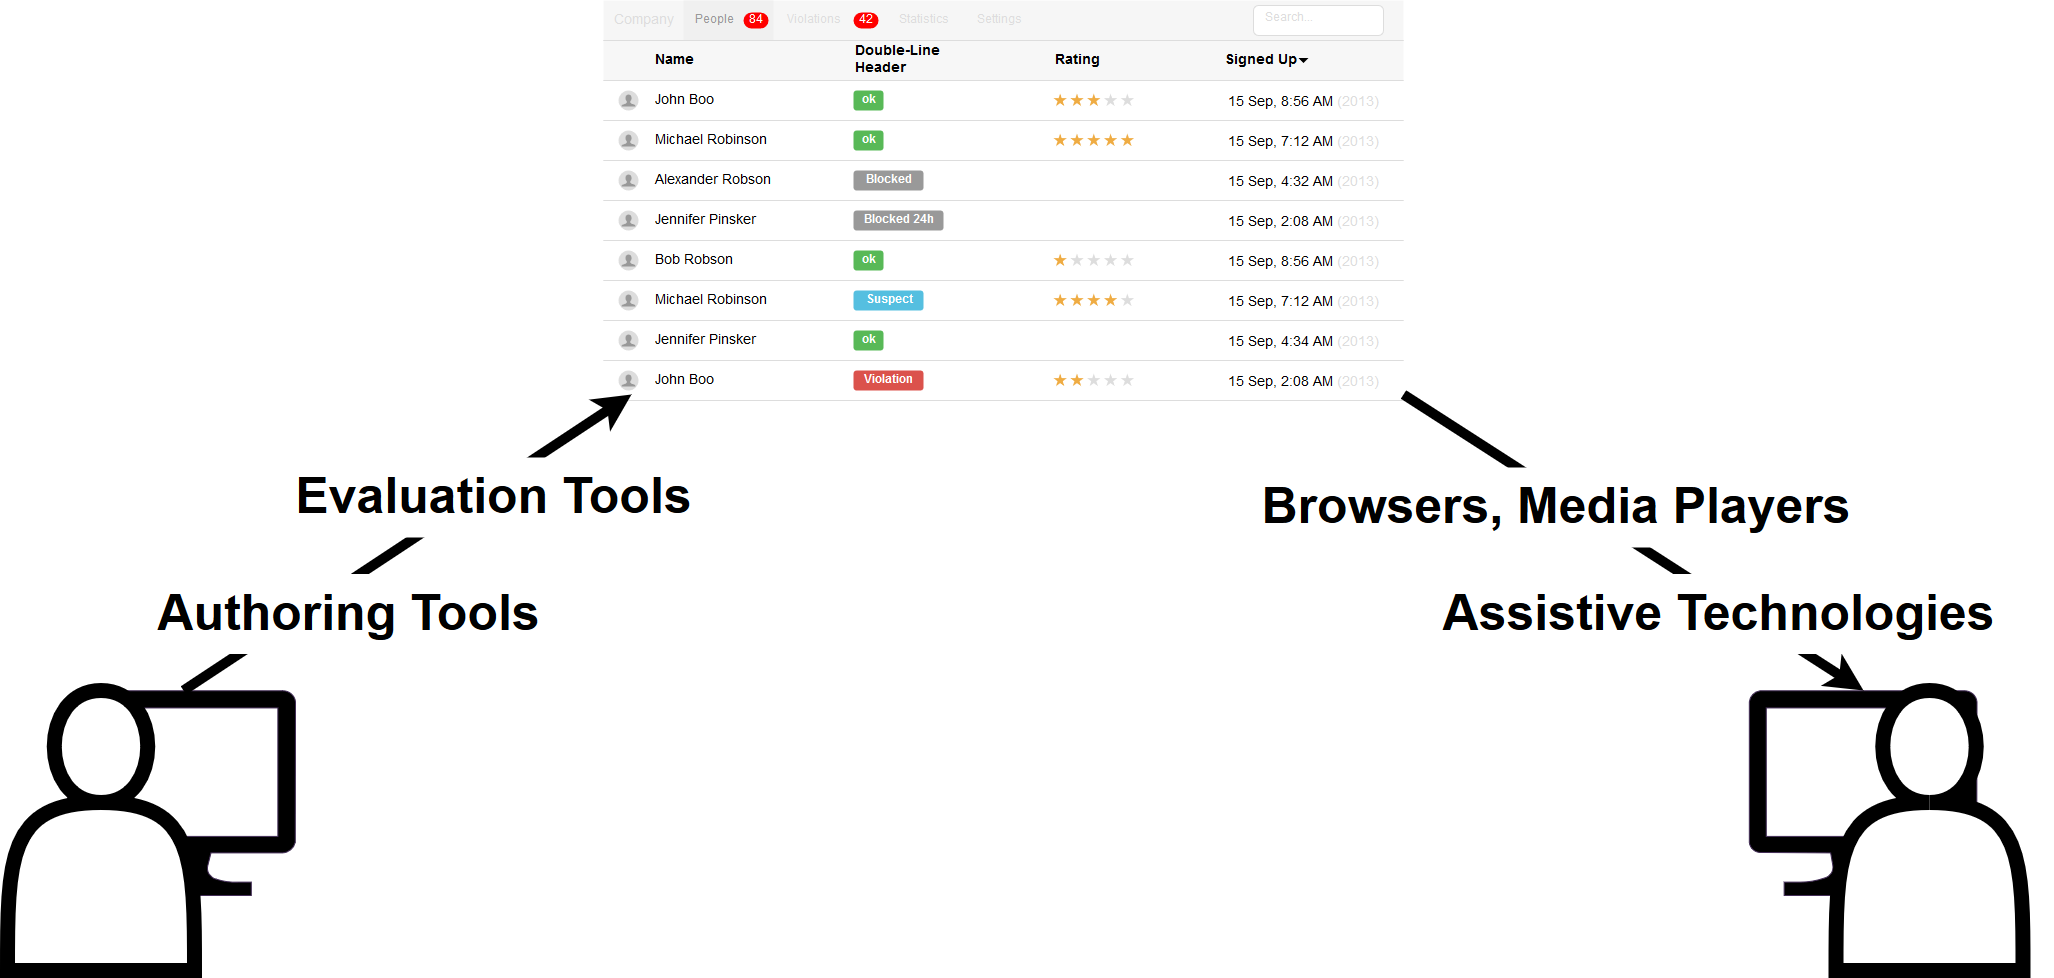
\includegraphics[width=8cm]{images/W3Components.png}
\centering
\end{figure}

\subsection{Web Accessibility Guidelines}
With the growing complexity of websites, and more web developers than ever, the World Wide Web Consortium (W3C) publish some guidelines and specifications around building accessibility into web pages.
These provide some guidelines in terms of the semantics to use, and how to define interactions, but even by following all of these there is still always a need to test on real users to ensure a website really is accessible to a range of people.

\subsubsection{WCAG}

The Web Content Accessibility Guidelines (WCAG) are part of a series of web accessibility guidelines published by the Web Accessibility Initiative (WAI) of the World Wide Web Consortium (W3C). WCAG 2.1 was published in 2018, and provides a much-needed update to the previous version published a decade earlier - mobile phone web browsing especially has increased a lot in the last 10 years and requires a new set of accessibility guidelines.

The WCAG are organised under 4 principles

\begin{itemize}
    \item Perceivable - users must be able to perceive the information being presented (it can't be invisible to all of their senses)
    \item Operable - users must be able to operate the interface (all interactions must be able to be performed by the user)
    \item Understandable - users must be able to understand the information presented and how to operate the interface
    \item Robust - users must be able to access the content from a variety of user agents, including current assistive technologies
\end{itemize}

Each of these principles has a set of testable criteria, and these can be met at 3 levels - A, AA and AAA, indicating a minimum, good, and high level of conformance, although it is not always possible to reach level AAA with all content types.

\subsubsection{WAI-ARIA}

The WAI-ARIA is a technical specification for making web pages accessible. WAI-ARIA defines some extra attributes

\begin{itemize}
    \item Roles - these define common structural roles on a web page such as \texttt{button}, \texttt{navigation}, \texttt{banner} and \texttt{tabgroup}, with a lot of overlap with HTML5 semantic elements
    \item Properties - these define the properties of elements that are important for meaning or semantics, such as \texttt{aria-required} to indicate if a form input is compulsory, or \texttt{aria-modal} to indicate that an element is modal when displayed
    \item States - these define a specific property type which indicate the current state of an element (these can be changed over time as opposed to properties), such as \texttt{aria-disabled} to indicate that a form input is visible but not editable
\end{itemize}

\subsection{Current Tooling}

\subsubsection{Tools for Development}

When aiming to develop an accessible website, there is no easy route - instead, it is important to keep accessibility in mind throughout the design and development process. The WCAG should be consulted when designing the site, and WAI-ARIA for guidelines on the semantics to use when developing the site.

As HTML5 is designed to be accessible, it is key to try and keep things as simple as possible, and not try to do "hacky" things when developing a site, such as using CSS to change the ordering of how elements show on a page. It is also important to use the designated HTML elements for each component on a page, such as using a \texttt{<button>} tag for a button instead of adding a \texttt{<span>} and styling it into a button.

Many web frameworks are built with accessibility considered, and so using frameworks like \textit{Bootstrap}, \textit{Turret}, \textit{Foundation} or \textit{Vanilla} for building the site and then evaluating and fixing any accessibility issues can also be a good idea.

A useful JavaScript library that is available is \textit{Ally.js}, which can be loaded into a JS project and provides a set of modules to help simplify accessibility challenges, such as setting specific ordering for tab focuses.

There are many tools that can also be used to evaluate a site's accessibility or even give live feedback to the developer while they are coding, these are discussed below.

\subsubsection{Tools for Evaluation}

Several well-made tools are available freely online to test and fix accessibility issues. \textit{Pa11y} provides a suite of tools to flag up accessibility issues, including tools that can be integrated into a CI workflow and provide live feedback on issues. \textit{HTML\_CodeSniffer} is a linter that allows different standards, such as WCAG, to be checked against code. \textit{WAVE} is another web accessibility evaluation tool that simply takes a URL and evaluates missing accessibility features.

It can be useful during development for a developer to simulate different disabilities to test the site, as this can flag up larger issues before testing on people who use assistive technologies. Testing with a screen-reader is also a good way to understand how a site will sound. \textit{JAWS} and \textit{NVDA} are two of the most commonly-used screen-readers, and most platforms also have native screen-readers that can be tested with - \textit{Voiceover} for Mac and iOS, \textit{Narrator} for Windows, and \textit{TalkBack} for Android.

It can also be useful to check how a site looks for colour-blind users. Some tools for this include \textit{Check My Colours} to check colour contrast, and \textit{Color Oracle} to simulate colour blindness.

A recent project from IBM is the \textit{Va11ys} project, which provides a range of code samples that allow a developer to test out different assistive technologies. These provide a good idea of how different accessible features should look as code, and how they should be interpreted by different assistive technologies.

Overall, we can see that there is a wide range of tools that are designed to help developers evaluate accessibility on their site and recognise issues before testing with real users, but not as many that focus on building accessible sites in the first place.

\begin{figure}[h]
  \centering
  \begin{subfigure}[b]{0.4\linewidth}
    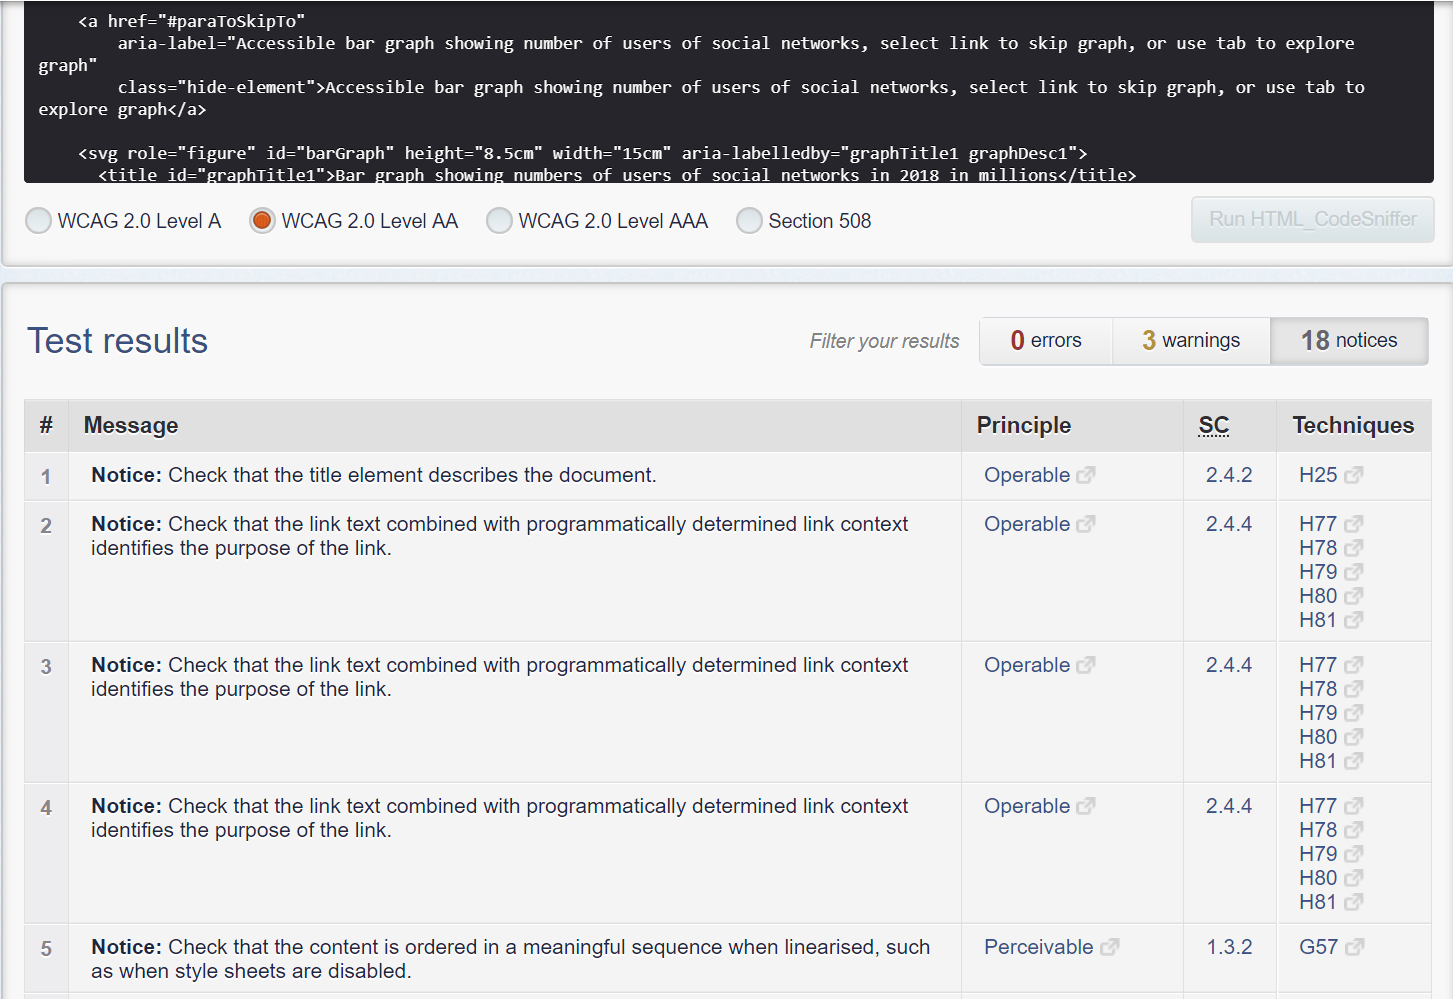
\includegraphics[width=0.9\linewidth]{images/HTMLCodeSniffer.PNG}
     \caption{HTML\_CodeSniffer}
  \end{subfigure}
  \begin{subfigure}[b]{0.4\linewidth}
    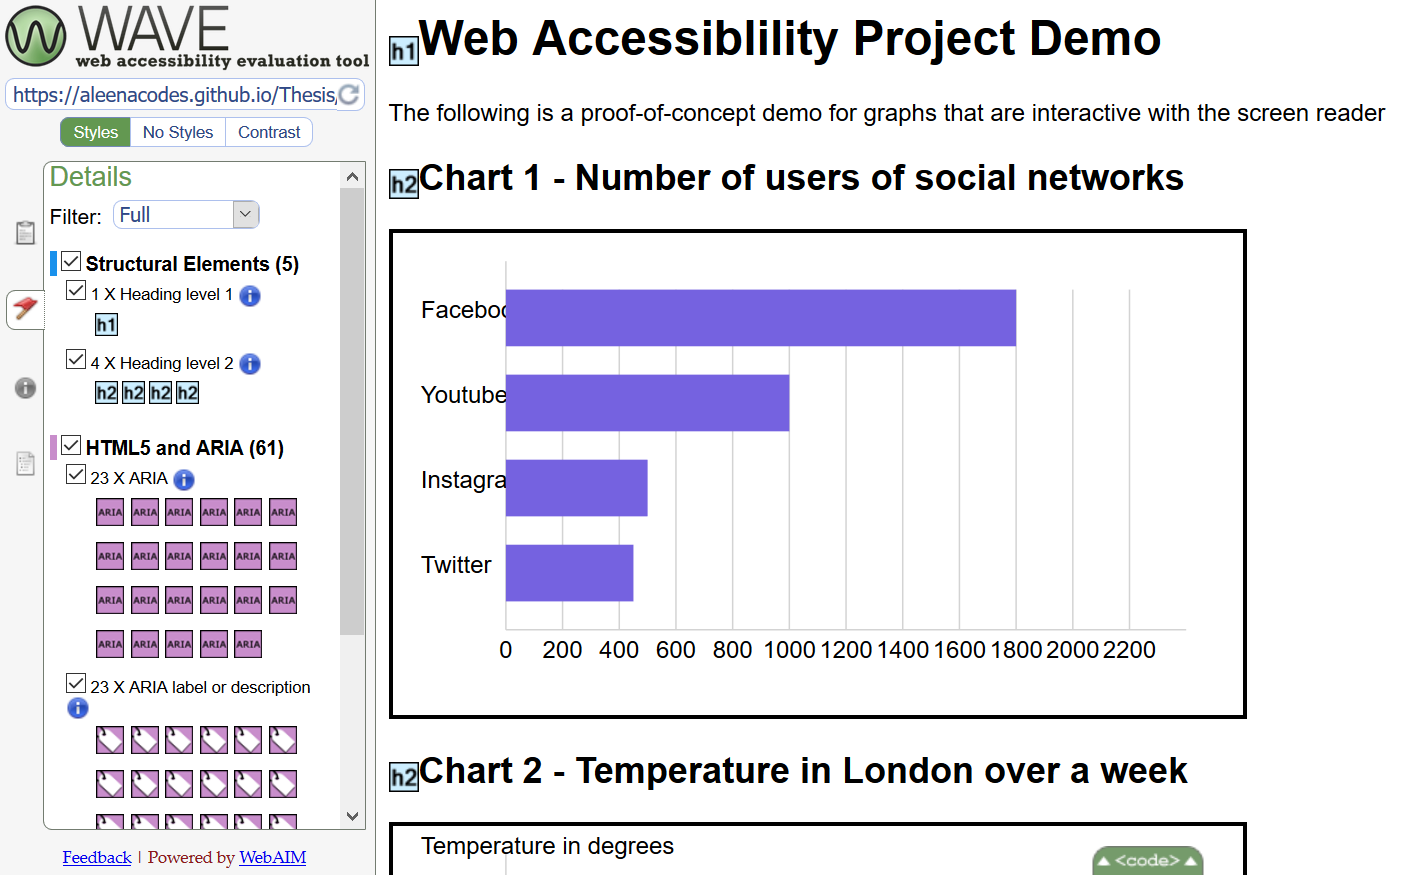
\includegraphics[width=\linewidth]{images/WAVETool.PNG}
    \caption{WAVE Evaluation Tool}
  \end{subfigure}
  \caption{Available tools to flag up accessibility issues}
  \label{fig:EvaluationTools}
\end{figure}

\subsubsection{Tools for Viewing Sites}

Users with disabilities tend to have two different approaches to interactions with the web

\begin{itemize}
    \item Assistive Technologies - using tools like screen-readers and voice recognition software to turn parts or all of a website into an understandable format
    \item Adaptive Strategies - making small changes to a site's format to make it easier to process, such as making fonts larger or turning captions on for videos
\end{itemize}

With each of these approaches, they require the developer to give correct layout/prompts on the site for them to work - the tables below detail this

\paragraph{Assistive Technologies}

\begin{center}
\begin{longtable}{|p{3cm}|p{5cm}|p{5cm}|}
 \hline
 Technology & Usage & Developer Notes \\ [0.5ex]
 \hline \hline
 Screen-Reader & Processes content on desktops and browsers, and converts it to audio or braille & Content needs to be structured properly and include labels and descriptions where needed, semantic HTML should be used as far as possible \\
 \hline
 Pop-up/Animation Blocker & Stops automatic pop-ups and redirection & Important info should not be included in pop-ups, and site browsing flow should not include redirection \\
 \hline
 Reading Assistant & Software that changes content presentation to make it more readable - this can include changing font and space, hiding parts of the page and reading text aloud & Different sections on a page should be used and labelled correctly, layouts should be responsive to font changes \\
 \hline
 Keyboard/ Mechanical Inputs & Many different custom keyboards are available - those with larger or illuminated keys, on-screen keyboard, sip-and-puff switches  & Content should be able to all be accessed via keyboard, and grouped together to allow fast navigation through a page \\
 \hline
 Mouse & Many different mice are available - touchpads, trackballs, joysticks & Different sections should be labelled, and clickable areas should be large enough to accommodate error margins\\
 \hline
 Eye Tracking & Monitors eye movements to control the mouse pointer, and blinking to click the mouse & Clickable areas on the page should not be too small \\
 \hline
 Voice Tracking & Uses voice commands to dictate text and issue commands & Different sections and clickable areas should be labelled well \\ [1ex]
 \hline
\end{longtable}
\end{center}

% LATER Left off - voice browser, braille display

\paragraph{Adaptive Strategies}

\begin{center}
\begin{longtable}{|p{3cm}|p{5cm}|p{5cm}|}
 \hline
 Technology & Usage & Developer Notes \\ [0.5ex]
 \hline \hline
 Captions & Text with verbatim recording of any speech or audio & Video platforms should be built to allow simultaneous captioning files to be run alongside video files \\
 \hline
 Screen Magnifier/Bigger Fonts & Pages can be magnified either be magnifying small sections or increasing font sizes overall & Page layouts should support text changes by using relative units for measurements and allow re-flow of text \\
 \hline
 Higher Contrast & Colours with significant contrast are easier to view for less-sighted and colour-blind users & Colour palettes should be decided in advance and tested via WCAG guidelines \\
 \hline
 Volume Control & Audio may need to be volume-adjusted or turned off altogether & Audio should not autoplay in order to not interfere with audio technologies, and options to adjust volume (including to 0) should be visible and accessible to both mouse and keyboard technologies \\ [1ex]
 \hline
\end{longtable}
\end{center}

% LATER - write more?

\subsubsection{Accessibility APIs}

In the early 1990s, assistive technologies would read what was on the screen and try to guess the functions of different elements and their states, e.g. by looking at class names of objects and seeing if they were highlighted. However, this was not always accurate and there was often some delay time between new features being introduced and assistive technologies being developed to recognise them. \cite{smashingAPIs}

In the late 1990s, accessibility APIs were introduced as a standardised alternative that provided a more reliable way to pass information to assistive technologies. For the first time, developers had the ability to provide information to assistive technologies in a predictable and consistent way.

Although this was a step up from the previous way of simply guessing information about pages, many early accessibility APIs still did not provide much structural information for the page, making it hard to understand how objects related to each other. New APIs were developed over the next decade, which were then able to provide information on page structure and rich text formatting.

Accessibility APIs represent objects in a UI, with each object able to be queried for information, including its role, name and current state. UI's are represented as a hierarchical tree, and many different elements are now able to be recognised, such as tabular layouts, and event notifications.

There are accessibility APIs on all major operating systems (both desktop and mobile), and browsers typically support the accessibility API for the platform they're running on, passing information about the browser and the rendered content onto the API.

One of the problems developers face is not being able to add to accessibility APIs, they can only write in semantics that will work well with an API but not directly influence the accessibility tree that an assistive technology will form.

A new (and still experimental) technology currently being worked on is the Accessibility Object Model (AOM). This aims to allow developers to directly provide information to assistive technology APIs via adding custom fields to elements on a page.

\section{Accessible Visuals}

Visuals are often used to quickly and easily convey large amounts of information to a reader. Data in tabular form can be hard to dig through, and graphs allow viewers to spot both simple and complex trends across many fields in one go and also draw their own conclusions about the data without having to see a large amount of raw data.

% LATER say something more about visuals

\subsection{Challenge with Creating Accessible Visuals}

Making pictures and graphs accessible on the web is often done by adding alt-text attributes to detail what an image shows. But it is easy to see why it would be hard to encompass the same level of detail in words for a graph than a viewer would be able to get visually

\begin{itemize}
    \item "Graph showing a stock price over time" - does not convey any actual information about the data in the graph
    \item "Graph showing an upward trend of a stock price" - conveys a bit more information about the data, but does not allow the user to get any sense of prices
    \item "Graph showing an upward trend of a stock price from $\pounds$ 60 to $\pounds$ 180 over 2 years" - gives some idea of prices and how fast they climbed but does not allow the user to see smaller details such as any dips in price
\end{itemize}

It is clear that in order for a text-based web user to have anywhere close to the insight that a sighted user would have from a graph, a large amount of long-winded description would need to be included with any graphs, which can be hard and long for a developer to write. Many developers try to account for this by also including the data in tabular form, which screen-readers can access and read. However, this is a clunky solution, especially as if the data was displayed graphically in the first place, it was likely not very easily consumable in tabular form.

\subsection{Current Solutions}

There are many JavaScript graphing libraries available for the web, most notably libraries such as \textit{Chart.js}, \textit{D3.js}, \textit{Highcharts} and \textit{Google Charts}.

Most of these libraries have some accessibility in mind in terms of alt-text and navigating via keyboard, but a big problem is consistency among browsers. Libraries like \textit{D3} and \textit{AmCharts} use SVG to form the images, and provide little ability for a user to navigate through these element-by-element.

The \textit{Highcharts} library offers some accessibility in terms of a custom module that can be loaded in. This provides the ability to show screen-reader users the data in raw form and to use high-contrast patterns in the graph. However, this still relies on the user to add sufficient alt-text to the graph and requires some custom set up from the user in terms of turning on a lot of different settings to enable keyboard navigation and other accessibility features.

\subsection{Aim}

In this paper, I will explore the creation of a JavaScript graphing library that comes with accessibility out-of-the-box.

The aim is to have a library that functions as a proof-of-concept for how web accessible graphs could be made. It will provide key accessibility features for several different types of graphs, with minimal work from the developer. In order to focus on accessibility and functionality, this library will be limited to a few common types of graphs.

\subsection{Technical Challenges}

One of the main technical challenges is making a solution that works out of the box to creates graphs that are usable for people browsing with and without assistive technologies. It is also key to note that while the WCAG provides some clear guidelines on how to make web content that is accessible to people with varying needs, it is still hard to get every use case due to the diverse needs of people using the internet.

When trying to provide all the information that sighted users would see via audio, it will also be important to keep a balance between providing relevant information and overloading the user. Providing too much information will be tedious for users who only want to understand the values and trends in a graph, and may also overwhelm a user, but providing too little information will result in less understanding about the graph for the user.

From a usability standpoint, it will also need to be easy for developers to use, but still be able to be customised enough that developers can create custom graphics to their liking while maintaining the same level of accessibility. Developers (understandably) lean towards using technologies that provide the solution they need with a minimal amount of work, so it will be important to keep the API functional but quick to invoke.

% \section{Related Work}

% LATER - write
% Some papers
% Some books
% Highcharts
% Amcharts
% Kendo UI
% Evocharts

\chapter{Design}

\section{Basics}

When thinking about the implementation, there were 3 main areas to think about

\begin{itemize}
    \item Types of graphs
    \item Information to present
    \item Colours and patterns
\end{itemize}

\subsection{Types of Graphs}

As I was trying to build a proof of concept, as opposed to a comprehensive library, I decided to focus on 3 different graph types - bar graphs, line graphs and pie charts. These chart types are some of the more commonly-used ones and are different enough to provide a varied proof of concept.
\newline
\begin{figure}[H]
  \centering
  \subcaptionbox{Bar Chart}[.3\linewidth][c]{%
    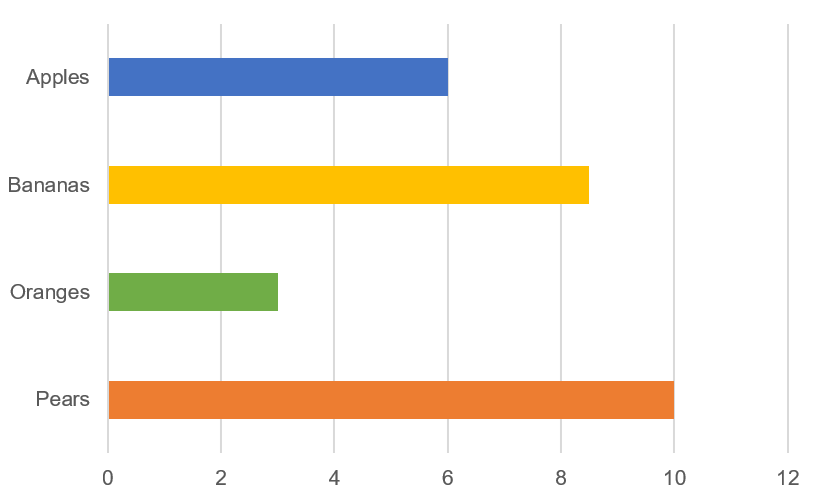
\includegraphics[width=.3\linewidth]{images/BarGraph.PNG}}\quad
  \subcaptionbox{Pie Chart}[.3\linewidth][c]{%
    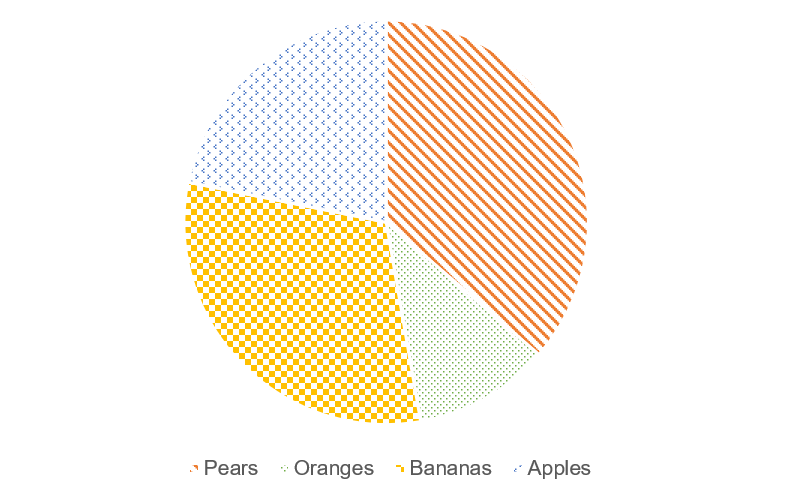
\includegraphics[width=.3\linewidth]{images/PieGraph.PNG}}\quad
  \subcaptionbox{Line Chart}[.3\linewidth][c]{%
    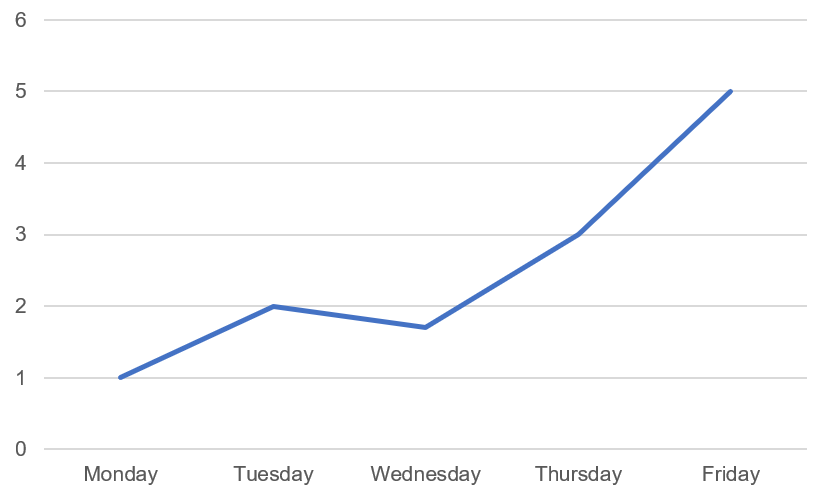
\includegraphics[width=.3\linewidth]{images/LineGraph.PNG}}
\end{figure}

\subsection{Information to Present}

Having spoken to some people who use screen-readers daily and observed them using these to browse web pages, it was clear that screen-reader users don't tend to listen to a web page in its entirety, instead scrolling through quickly to find information that they need.

In order to accommodate this, I aimed to create labels for the chart that were not too verbose, and which had the most pertinent information at the start of the label. This would mean that if the user was trying to find a particular data point, they would be able to move through each data point quickly in order to accomplish this.

I felt that the key information to present were the headings and values of the data, and also to highlight some broader trends without overloading the user with too much detail.

\begin{figure}[h]
\caption{Examples of possible labels}
\centering
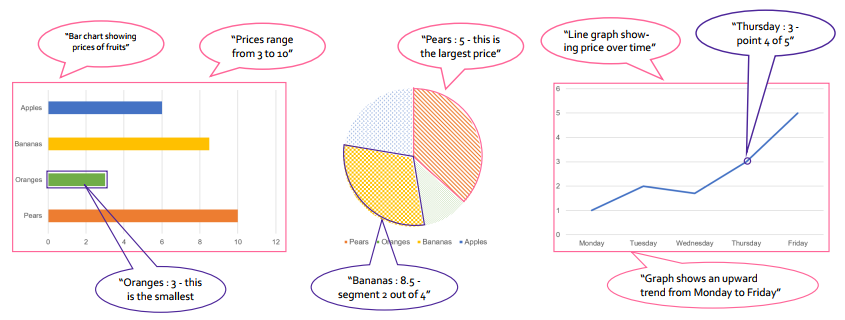
\includegraphics[width=0.9\textwidth]{images/GraphDesignWithReadouts.PNG}
\end{figure}

\subsection{Colours and Patterns}

Use of colour and pattern is important for users who are partially-sighted or colour-blind, and a common method found in many websites and games that rely on colour is to have a "colour-blind" mode which changes different colours to be different patterns instead.

The WCAG require a minimum level of contrast of \textit{4.5:1} between colours to fulfil criterion \textit{1.4.3 - Minimum Contrast}, and so I used this as a guideline to select colours.

I also aimed to combine the use of contrasting colours with different patterns as well, as these would help users distinguish between different sections. Another thing that is known to be helpful with partially-sighted and colour-blind users, is to allow some white space between corresponding elements to help the user better distinguish between elements such as bars or segments on charts.

When building a colour palette, I aimed to have 6 different colours in my colour palette, which would have a good amount of contrast with each other. Since I was making a graphing library, I initially thought of using a \textit{Brewer Palette} - colour combinations that are specifically selected for their properties for use in data visualisation and information design. These colours are selected based on human perception around which colours seem associated with each other, and so a \textit{Qualitative Brewer Palette} seemed like a good choice for the graphs I was creating. However, I found that these colours had little contrast between them by WCAG standards, and so would not be suitable for my use.

In order to check the contrast between each colour, I used a colour contrast-checker from the design agency \textit{EightShapes} to load in multiple colours and see the contrast level between each colour.

\begin{figure}[h]
\caption{Checking colour contrast with the EightShapes contrast checker tool}
\centering
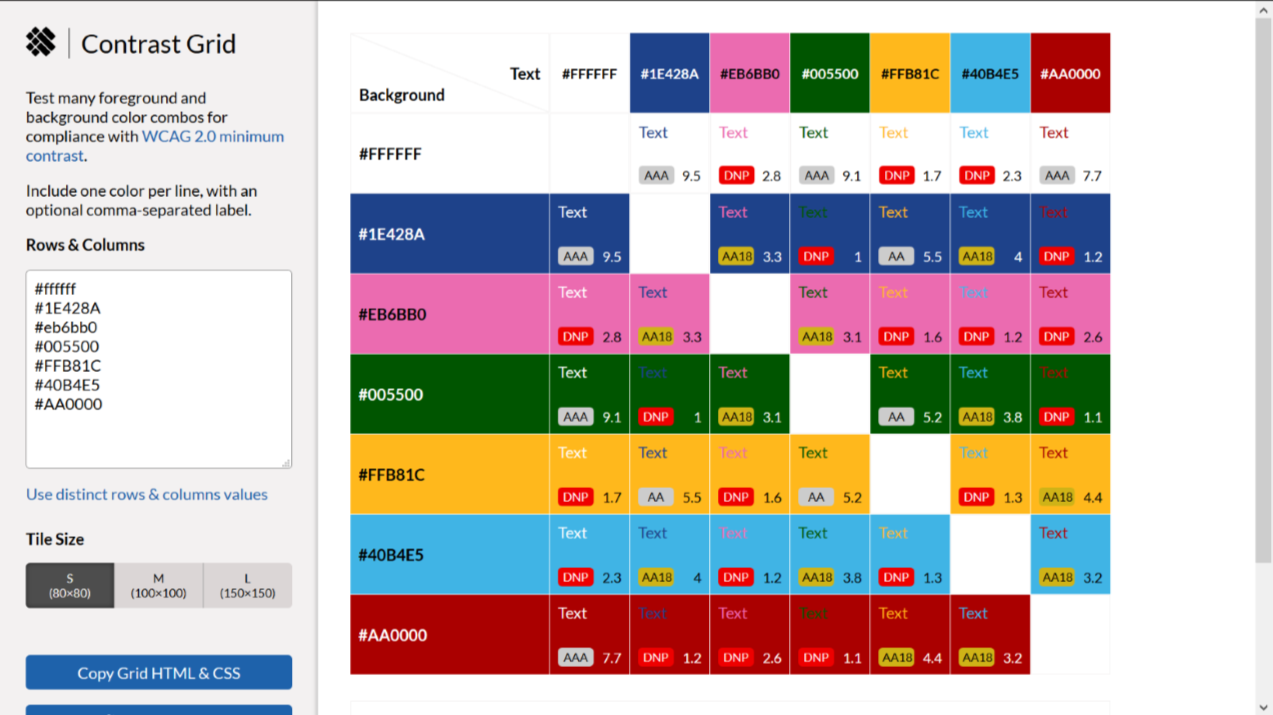
\includegraphics[width=0.5\textwidth]{images/EightShapeColourChecker.png}
\end{figure}

With this, I was able to build a palette of 6 colours which had a fairly high contrast level between most of the other colours (i.e. 3 or more). However, it proved very hard to find colours that had a high enough contrast between all other colours in a palette, and so I decided to keep the current palette and simply make sure that neighbouring colours were high contrast.

\section{Accessibility Tree}

When looking at web accessibility, a key concept is the accessibility tree - a tree structure created from a web page's DOM, which assistive technologies are then able to interact with. One of the major technical issues with this project was that different web browsers may generate slightly different accessibility trees from the same HTML code and different assistive technologies may also interpret the same accessibility tree differently. Thus it would be hard to make a solution that worked across all of the common assistive technology/browser/operating system combinations.

% LATER - diagram of how assistive tech uses accessibility trees?

Many browsers, such as Mozilla Firefox, provide tools to directly view the accessibility tree, and so I aimed to use syntax to create as clean an accessibility tree as possible (and by extension the DOM would also be clean).

The WAI-ARIA standards provide a set of roles, states and properties that can be given to HTML elements, along with a way to label these, and so I aimed to use these extensively to build an accessibility tree with correct elements and labels

\section{Library Design}

When building the JavaScript library, since this was a proof-of-concept, I aimed to create a fairly simple API for the developer, in which the page \texttt{div} in which to create the chart, the chart type, and data source (a local file) could be specified. Along with this, the chart title and units of data would need to be specified, in order to generate the metadata for the chart correctly.

% LATER - in which the page \texttt{div} in which to create the chart - sentence incomplete

\chapter{Implementation}

\section{Implementation of syntax}

\subsection{Using SVG}

The most common way of generating images in web pages is using SVG, either embedded (included from an external file) or inline. SVG allows geometric shapes to be specified and positioned, and so it was an obvious choice for this project.

Inlining SVG provides more predictable results and better control over properties than adding in SVG files with a \texttt{<img>} or \texttt{<use>} tag. This is because the SVG source is then directly available in the DOM, which is exposed by the accessibility API used by assistive technologies.

While SVG has been around for a while (since 2001), there has recently been a push towards a more modern version, resulting in a new specification for SVG 2 being released in 2016.

One of the new features in this specification is the abilities to add \texttt{tabindex} to SVG elements (such as shapes or text). This is useful, as previously the only way to make elements in an SVG that were focusable by keyboard, was by including an HTML element that supported this, such as the \texttt{<a>} tag.

Although the W3C has released this specification, the onus is on the makers of a browser to implement these new features in their browser. Thus far there has been little uptake on this, with most browsers only implementing part of the specification, including accessibility-forward browsers such as Mozilla Firefox. Hence it is not necessarily an easy task to make a solution that works consistently across multiple web browsers (a problem common in all branches of web development).

\subsection{HTML Layout}

HTML, by virtue of being a markup language that defines only the structure of a web page, is set up to generate a DOM that is true to the page's visual structure, and as web development has progressed, new elements have been added to account for commonly-used parts of a web page.

HTML5 introduced the concept of a web page having "sections", with a new \texttt{<section>} tag that could be used to define a page's sections, as opposed to the more ambiguous \texttt{<div>}.

Sections are able to be nested within each other, giving the same type of structure as the original \texttt{<h1>, <h2>, <h3>} etc. tags created. However, it is not always desirable to have every section's children included in the outline of its parent.

A sectioning root is an HTML element that can have its own outline, but the sections and headings inside it do not contribute to the outline of its ancestor. The sectioning root \texttt{<figure>} is the key one that I used in my development, to create an element that was able to have many children (i.e. axis, data points etc.) and not create a lot of excess outline in the DOM for the parent section.

% picture illustrating sectioning root and non-sectioning root?

\subsection{ARIA syntax}

As discussed before, I aimed to create as much of the accessibility tree as possible from using inbuilt HTML properties (e.g. using \texttt{<h1>}) for headers as opposed to adding an ARIA role to achieve this. ARIA provides custom roles for elements, but many of these double up with those assigned to native HTML elements (such as \texttt{role="button"}, which can also be assigned by using \texttt{<button>}). However, many of the ARIA roles that double up with HTML have to also have extra parts defined, such as making the element focusable and defining event handlers, so it is not usually recommended to use an ARIA role when there is a native HTML element available.

While I was initially using the element \texttt{<figure>} as the parent element, I found that it was easier to use the ARIA role \texttt{figure} directly as an attribute of the \texttt{<svg>} tag, thus making it act as a \texttt{<figure>} tag when it came to creating the DOM, and also meaning that it showed up directly as \texttt{figure} in the accessibility tree, as opposed to being an only-child \texttt{svg} nested inside a \texttt{figure}.

I used the SVG properties \texttt{title} and \texttt{desc} to create a title and description for the chart. A lot of browsers were able to use only this to correctly label the figure in the accessibility tree, but I also encoded this in using ARIA.

The ARIA property \texttt{aria-labelledby} is used to create a label that is displayed in the accessibility tree only, thus making it only visible to people using assistive technologies, and not available to those browsing the web normally.

The \texttt{aria-labelledby} property, alongside the \texttt{aria-describedby} property identify the element(s) are used to label and describe the current element (\texttt{describedby} is intended for a more verbose description).

In my case, I found that \texttt{aria-describedby} did not work very consistently across browsers, and so it was largely pointless in most use cases. Instead, I doubled on \texttt{aria-labelledby} to include both the title and description.

Through using both the \texttt{<title>} and \texttt{<desc>} tags for the SVG, and using \texttt{aria-labelledby} to also link these, I covered most browser/screen-reader combinations for reading this out.

Since the reader was going to browse through the contents of the SVG, I also used \texttt{aria-hidden} to hide the excess parts of the chart, such as the lines and labelling for each axis. This was an effective way to keep these out of the accessibility but keep them in the DOM, so visible on the page. Figure \ref{fig:HTMLATComparison} shows how \texttt{<title>} and \texttt{<desc>} tags are included in the corresponding nodes in an accessibility tree, and how elements with the \texttt{aria-hidden} attribute are not included when constructing the accessibility tree.

\begin{figure}[h]
  \centering
  \begin{subfigure}[b]{0.8\textwidth}
    \centering
    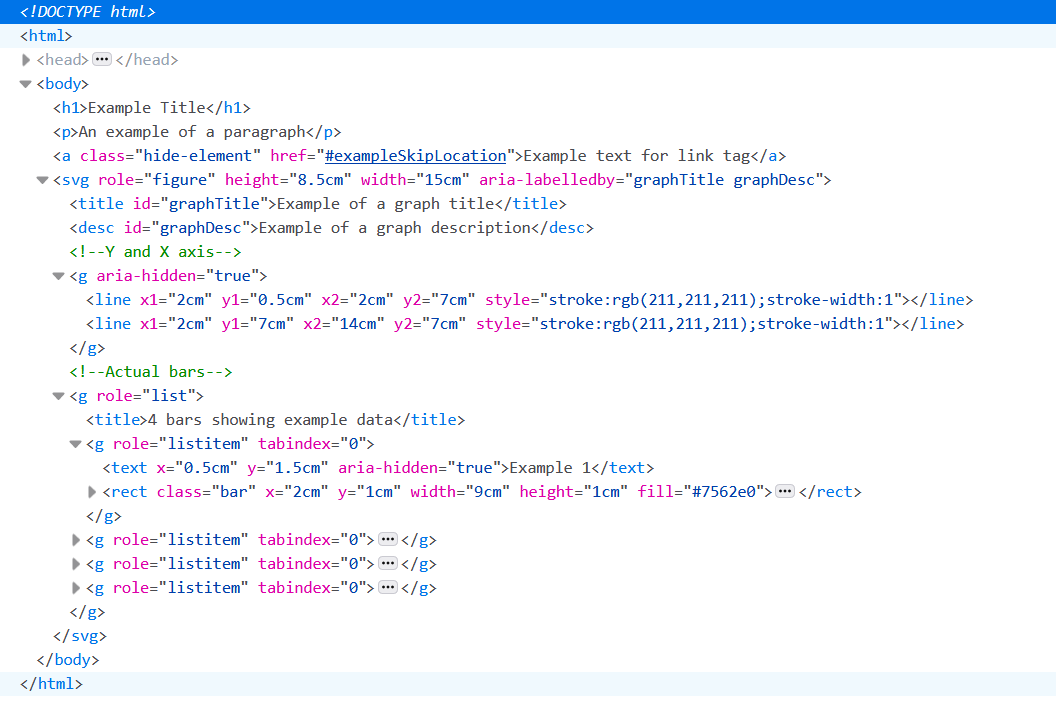
\includegraphics[width=\linewidth]{images/ExampleHTML.PNG}
     \caption{HTML markup}
  \end{subfigure}
  \begin{subfigure}[b]{0.8\textwidth}
    \centering
    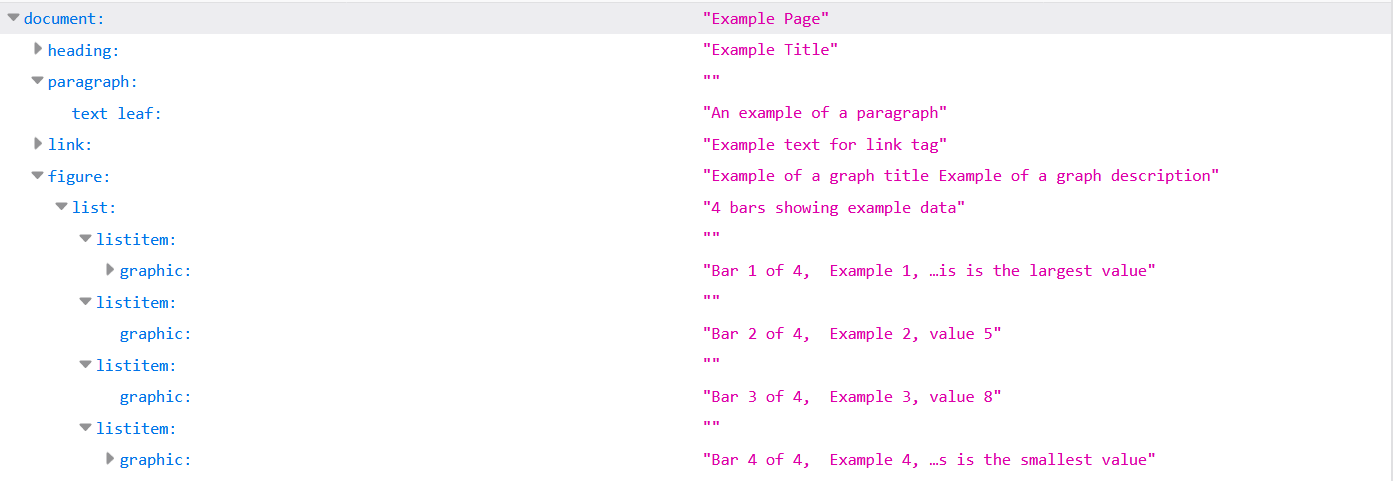
\includegraphics[width=\linewidth]{images/ExampleAccessibilityTree.PNG}
    \caption{Accessibility tree}
  \end{subfigure}
  \caption{An example of how HTML markup would produce an accessibility tree}
  \label{fig:HTMLATComparison}
\end{figure}

In order to make each data point able to be accessed individually, I added a \texttt{tabindex=0} property to each data point. This made each of these elements focusable and thus added them to the order in sequential keyboard navigation, letting them be accessed by using the \texttt{[Tab]} key on a keyboard.

I also grouped the data points in an SVG group \texttt{<g>} and gave this an ARIA role of \texttt{list}, along with a \texttt{<title>}. This meant that when a screen-reader came across the list it would read out the title. I then added each data point as an SVG group of its own, with an ARIA role of \texttt{listitem}, and a \texttt{<title>}, which the screen-reader would read out on focussing on each list item. Setting up the chart as a \texttt{list} containing a set of \texttt{listitem} also meant that users of technologies that have other shortcuts for navigating lists could also use these.

\begin{figure}[h]
\caption{Using the \texttt{<title>} tag and ARIA roles}
\centering
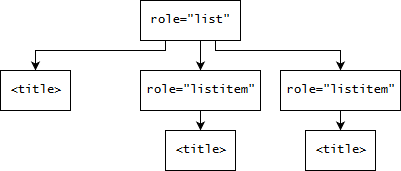
\includegraphics[width=0.5\textwidth]{images/listitemnesting.png}
\end{figure}

\subsection{WCAG}

I also had the Web Content Accessibility Guidelines (WCAG) in mind when implementing this, and so I had to implement a few things to satisfy the guidelines, most notably a \textit{Bypass Block} mechanism as specified in success criterion \textit{2.4.1}. This meant adding a simple link that let the user skip past the graph entirely if they chose to, as opposed to having to listen to the entire read-out of the graph.

Although many of the criteria didn't apply to this project, especially those to do with an entire web page, or time-based events, some of the other criteria also had to be implemented in terms of syntax, such as

\begin{itemize}
    \item \textit{Criterion 1.1.1} - Providing non-text Content - this was a major focus of my implementation, and done using \texttt{aria-labelledby} and \texttt{aria-label}
    \item \textit{Criterion 1.3.1} - Info and Relationships - by creating the data points as a \texttt{list} with corresponding \texttt{listitem} elements, the nature of the relationship of these was kept clear
    \item \textit{Criterion 2.1.3} - Keyboard - by making elements focusable (via adding \texttt{tabindex=0}) all the content was operable through keyboard interface
    \item \textit{Criterion 2.5.3} - Label in Name - all the generated \texttt{aria-label} labellings matched the visual information that was displayed on screen
    \item \textit{Criterion 3.1.5} - Reading Level - the \texttt{aria-label} on each data point was kept short and simple in order to make it clearly understandable by users of all reading levels
    \item \textit{Criterion 4.1.2} - Name, Role, Value - all roles were set using the standard \texttt{role=} syntax or auto-generated from the user of HTML tags, so any external technologies (such as assistive technologies) would be able to extract this information
\end{itemize}

\subsection{Expanding for compatibility in Safari/MacOS}

When testing on Windows machines with the two most popular screen-readers - \textit{NVDA} and \textit{JAWS}, the system of having a \texttt{<title>} tag for each \texttt{listitem} meant that when the user focussed on each element the specified \texttt{title} was read out.

However on MacOS with the native screen-reader \textit{Voiceover} this did not work at all, with no label being read out. This was a good example of large inconsistencies between browsers, even amongst the more well-maintained browsers.

In order to have the graph function as normal, I had to add an extra layer of labelling that \textit{Voiceover} would pick up on. For this I used the \texttt{aria-label} attribute to label each data point, with the same info as specified in the \texttt{<title>} tag. The \texttt{aria-label} attribute is similar to \texttt{aria-labelledby} but uses a direct string to read out, as opposed to referencing another HTML element as a label. It was suitable for use here as the label was fairly short, but would not have been suitable for a long-form description to be included.

\section{Implementation of library}

\subsection{Basic Structure}

I initially began with a hard-coded HTML prototype to figure out the syntax and run some user testing with. Once I had decided on the HTML syntax that I would use, I then proceeded to package this into a JavaScript library which would be able to produce the same graphs with any provided dataset.

I was keen to not have any external dependencies for the library, as JavaScript libraries are well-known for quickly growing very large as multiple levels of dependencies are loaded for a single small function. Thus I wrote only in "Vanilla" JavaScript - plain JavaScript without any functions from third-party libraries.

While a JavaScript library can just be included as a single file with all functions in it, with each required function just called directly, in order to avoid nameclashes with other libraries, I put the required function into a global object, which then served as the unique namespace for the library.
\newline
\begin{lstlisting}
var accessibleGrapher = {
    makeAccessibleChart: function(selector, chartInfo) {

    ...
  }
}
\end{lstlisting}

\subsection{Pulling in Data}

As the library was intended for small amounts of data, it would have been possible to simply require the user to send an array of data in the function call. However, the convention in graphing libraries is to allow an external file to be handed in, either locally or via an API call.

Since I was building a proof-of-concept library, I opted to only provide the option for loading in a local JSON file, although extending the library to load a file via an API call would not require too much extra code in the library.

The file was loaded in via an \texttt{XMLHttpRequest} - a standard object provided by the browser's JavaScript environment that allows data transfer between a web browser and web server.

\begin{figure}[h]
\caption{Parts of an XMLHttpRequest execution}
\centering
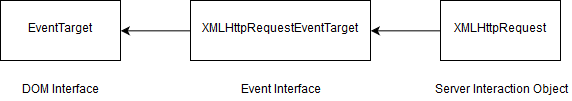
\includegraphics[width=0.5\textwidth]{images/XMLHttpRequest.png}
\end{figure}

I wrote a small function that would take the file path for the data that was provided by the developer, and run a callback to find and load in the file, and then create the graph.

\begin{lstlisting}
function loadJSONandMakeChart(fileName, callback) {
  var reqObj = new XMLHttpRequest();
  reqObj.overrideMimeType("application/json");
  reqObj.open('GET', fileName, true);
  reqObj.onreadystatechange = function () {
        if (reqObj.readyState == 4 && reqObj.status == "200") {
          callback(reqObj.responseText);
        }
  };
  reqObj.send(null);
}
\end{lstlisting}

The use of callbacks is standard in JavaScript usage on the web and allowed the code to run in the correct order, i.e. only making the chart once data was loaded in. The call was made as follows

\begin{lstlisting}
loadJSONandMakeChart(chartInfo["fileName"], function(response) {
  var chartData = JSON.parse(response);
  makeChart(chartData, chartInfo, selector);
});
\end{lstlisting}

This provided a small callback to the data loading function, which would load data, use JavaScript's standard \texttt{JSON.parse} method to turn the JSON into a JavaScript object, and then run a \texttt{makeChart} function once the data was completely loaded and parsed correctly.

This data, along with the chart information that the developer supplied in the function call was then passed to another function to determine the type of chart and then passed onto the final function to generate the correct type of chart.

\subsection{Interacting with the Webpage}

The \texttt{Document} interface represents a web page in a browser, and is the standard way to query and modify a page's DOM. The method \texttt{document.getElementById} provided a way to get the unique \texttt{Element} object associated with a single HTML element on a web page, specified by a unique \texttt{id} attribute on the element.

% LATER - diagram of HTML document interface

The methods \texttt{document.createElement} and \texttt{document.setAttribute} provided standard way to create new HTML elements and add required attributes onto them.

However, since SVG is part of an XML namespace (as opposed to the pure HTML namespace), it has to be created via an extended function \texttt{document.createElementNS}. The DOM 2 specification (now almost 20 years old) tackled the issue of multiple XML namespaces having identical tags with each other or with HTML, and so the \texttt{createElementNS} method allows the developer to specify the namespace URI for an element.

\begin{lstlisting}
var newSVG=document.createElementNS("http://www.w3.org/2000/svg","svg");
\end{lstlisting}

I also used the corresponding \texttt{document.setAttributeNS} method in my library, as this is a more future-proof way to code and allows consistency between \texttt{setAttribute} calls even if a namespace isn't specified.

The bulk of the graph-making functions were simple translations from the previously-created HTML to creating those elements as HTML elements via JavaScript and setting the attributes as required. SVG also has many alignment properties for text that allowed me to position things without using CSS, such as \texttt{text-anchor} and \texttt{dominant-baseline} for the SVG \texttt{<text>} tag.

The information for the ARIA labels was mainly able to be made by looking through the provided data to get properties such as the number of elements, and the smallest and biggest elements. These, combined with the \texttt{"units"} property that the developer put in the method call were used to create labels that read like natural language.

% LATER - some example of the natural language labels?

\subsection{Making Readable Axis}

For the bar and pie charts (but not the line chart) the data needed to be sorted by the value, and so a small helper function handled this.

\begin{lstlisting}
function sortData(array){
  sortedArray = array;

  sortedArray.sort(function(a,b){
    if(a.value == b.value)
        return 0;
    if(a.value > b.value)
        return -1;
    if(a.value < b.value)
        return 1;
  });

  return sortedArray;
}
\end{lstlisting}

When hand-coding the initial graphs I had been able to make axes that provided natural spacing between points (e.g. going up in 5's or 10's) but when creating the library, if the smaller and bigger data points weren't rounded like this, then the axis could become awkward and not very readable to the sighted user

To make more readable axis, I also had a helper function to round the last number on the axis to the next relevant power of 10, which would shift the axis to a more natural-looking spacing.

\begin{lstlisting}
function findChartEndNum(dataEndNum){
  lengthofNum = dataEndNum.toString().length;
  divNum = 1;

  if (lengthofNum >= 2){
    divNum = Math.pow(10, (lengthofNum-1))
  }

  endNum = Math.ceil(dataEndNum / divNum) * divNum;
  return endNum;
}
\end{lstlisting}

\begin{figure}[h]
  \centering
  \begin{subfigure}[b]{0.4\linewidth}
    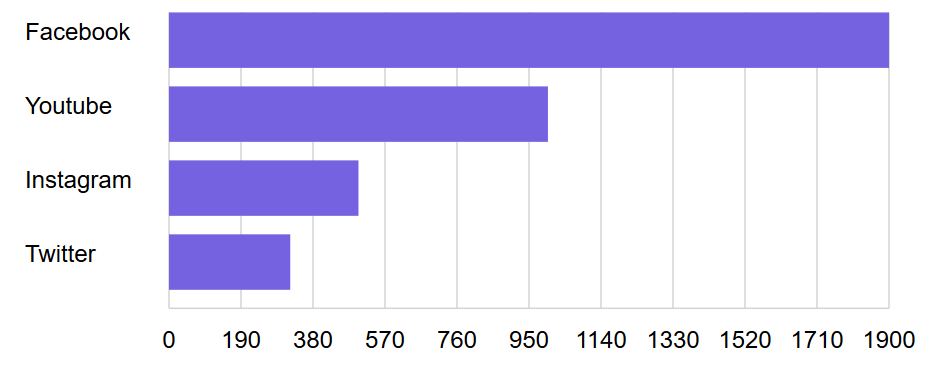
\includegraphics[width=\linewidth]{images/awkwardAxis.PNG}
     \caption{Awkward axis spacing}
  \end{subfigure}
  \begin{subfigure}[b]{0.4\linewidth}
    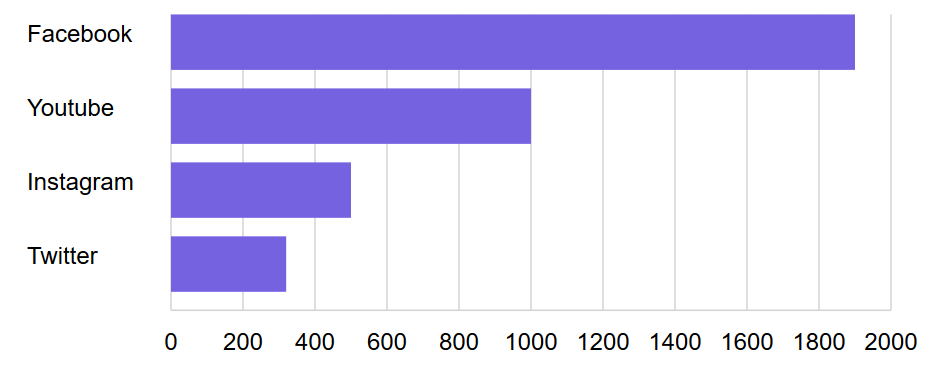
\includegraphics[width=\linewidth]{images/lessAwkwardAxis.PNG}
    \caption{More intuitive axis spacing}
  \end{subfigure}
  \caption{Before and after axis}
  \label{fig:Awkwardsaxis}
\end{figure}

\subsection{Calculating Trends and Other Mathematics}

For the line graph, I wanted to calculate a general trend as part of the overarching graph description, as this is something that a sighted user would be able to tell quickly upon seeing a graph.

In the spirit of not wanting to use any external libraries, I wrote up a JavaScript version of the \textit{Least Squares Method} -  an approach in regression analysis that estimates the relationship between a set of points, in this case the points on the line graph.

The algorithm works to find the "line of best fit" through a set of 2D points, by finding the line that minimises the square of the residuals, i.e. the error between the line's predicted value and the actual observed value.

The typical Least Squares algorithm takes in a list of points as $(x,y)$ co-ordinates, and so I used the SVG \texttt{width} and \texttt{height} to get the data point position, and then calculated its position relative to the bottom left corner (as opposed to the top left which SVG uses for its measurements).

When it came to drawing bar and line graphs, the mathematics was relatively simple to take in the data and draw \texttt{<rect>} of the correct width or \texttt{<circle>} at the correct position. However, drawing a pie chart required more maths to calculate and draw each segment correctly.

For the pie chart SVG, I added a \texttt{viewbox} property to the SVG. This meant that regardless of the actual size in pixels on the page, the relative measurements would stay the same when specifying measurements for each individual element to draw.

In order to draw the pie charts, I first calculated corresponding percentages for each data point out of the total of all values and then used this to work out the point on the circle for the edge of each segment.

\begin{lstlisting}
var x = radius * Math.cos(2 * Math.PI * percent);
var y = radius * Math.sin(2 * Math.PI * percent);
\end{lstlisting}

\begin{wrapfigure}{r}{0.25\textwidth}
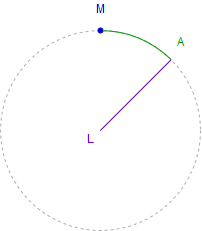
\includegraphics[width=0.9\linewidth]{images/DrawingArc.png} 
\caption{Drawing an SVG arc}
\end{wrapfigure}

This could then be adjusted to the correct position relative to the centre of the circle, and then drawn using the SVG \texttt{<path>} attribute. The path had 3 parts

\begin{itemize}
    \item \texttt{M} - \textit{Move} to the first point on the segment
    \item \texttt{A} - Draw and \textit{arc} to the next point on the segment
    \item \texttt{L} - Draw a \textit{line} to the centre of the circle
\end{itemize}

Although this method only drew two lines of the segment, SVG filled in the third automatically (as a straight line from the centre back to the first point of the segment), and this area could then be filled in like a normal shape.

% LATER - rewrite once implemented

\section{Limitations}

Although the library provides a proof-of-concept for generating 3 different types of graphs from provided data, there are still some key limitations in this approach.

A key concept in accessibility is that just because something is available to a user, it doesn't necessarily mean that it is accessible. In this case, this solution will be inefficient for large amounts of data, as although it could still provide a solution which would allow a user of an assistive technology access to all the information, it would quickly become tedious to have to listen to so much data, and it would also create a less-readable visual version of a graph.

It is also very hard to truly make a solution that is accessible to everyone, as disabilities come in a wide variety of effects and severities. When it comes to things such as the labels on the graphs, making descriptions that are simple enough for people with cognitive disabilities to be able to understand, may result in taking away too much detail. The current solution provides fairly simple labels but these could be extended slightly to provide other useful information for the user.

The solution uses the \texttt{[tab]} key to navigate through the graph, but for some users, the \texttt{[tab]} key may be associated with navigating through clickable links, and so this can be confusing. There is currently no standard way to allow arrow key navigation through an SVG, but it is possible to create a section of a web page with the ARIA role of \texttt{application}, which allows custom keystroke actions to be specified. However, this can cause other compatibility issues due to the variety of assistive technologies that may use a page, and this is considered bad practice to do unless done with great care.

\chapter{Evaluation}

\section{Study}

\subsection{Study Design}

% LATER - picture of demo
% \begin{wrapfigure}{r}{0.4\textwidth} %this figure will be at the right
%     \centering
%     \caption{Demo page}
%     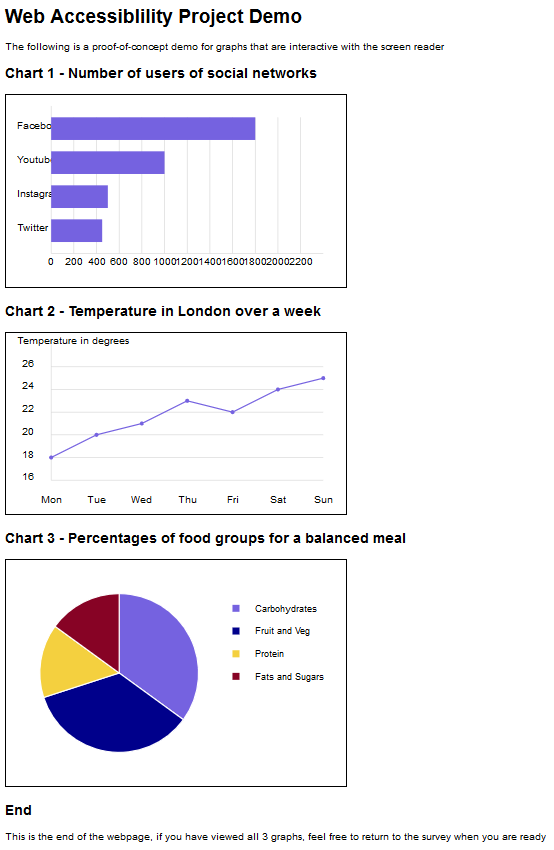
\includegraphics[width=0.35\textwidth]{images/Demo.PNG}
% \end{wrapfigure}


With the type of target market that was intended, it was important to test my solution on real-life users, especially those who use audio assistive technologies such as screen-readers, as there is a wide variety in the way that blind and partially-blind users navigate web pages based on operating system/browser combinations and also just preference.

As screen-reader users are a small group compared to all web users, I intended to try to run only a small round of user testing - around 5 or so users. Overall I had 7 users in the study. I tried to keep the study short for the user (less than 30 minutes) and so the demo was only one of each type of graph, and both surveys combined were 11 questions, mainly multiple-choice. The study consisted of 3 main parts. 

\begin{itemize}
    \item Background questions
    \begin{itemize}
        \item Before showing any content to the user I asked some background questions about their current software, and their usage of screen-readers
        \item There were also questions on their current perception around if they found images and charts on web pages accessible
    \end{itemize}
    \item Interactive demo
    \begin{itemize}
        \item The demo consisted of a simple web page made with the 3 graphs displayed and some headings in between
        \item The user could browse around the page in their own time and take however long they wanted on any specific section, provided they view all 3 graphs
    \end{itemize}
    \item Post-Demo questions
    \begin{itemize}
        \item The questions asked after the demo was shown focused on whether the user understood the graph data and how they felt the keyboard navigation was
        \item The user could also provide any other qualitative feedback that they wanted to, such as notes on what changes they would have liked
    \end{itemize}
\end{itemize}

\subsection{Results}

The background questions had results as follows

\begin{figure}[H]
  \centering
  \begin{subfigure}[c]{0.4\linewidth}
    \centering
    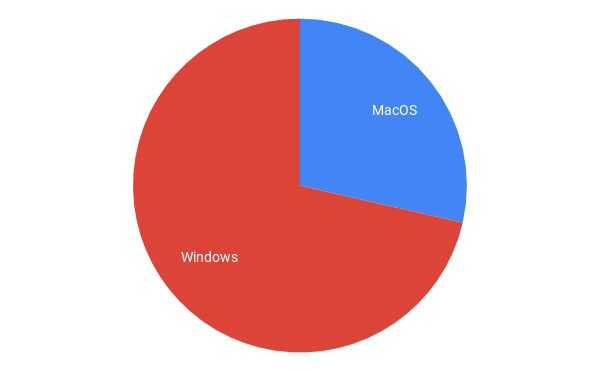
\includegraphics[width=0.75\linewidth]{images/OperatingSystem.png}
     \caption{What Operating System are you using?}
  \end{subfigure}
  \begin{subfigure}[c]{0.4\linewidth}
    \centering
    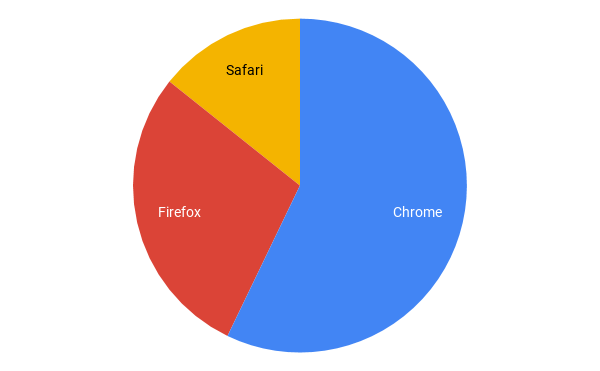
\includegraphics[width=0.75\linewidth]{images/WebBrowser.png}
    \caption{What web browser are you using?}
  \end{subfigure}
  \caption{Questions about software used}
  \label{fig:backgroundquestions}
\end{figure}

\begin{figure}[H]
  \centering
  \begin{subfigure}[c]{0.3\linewidth}
    \centering
    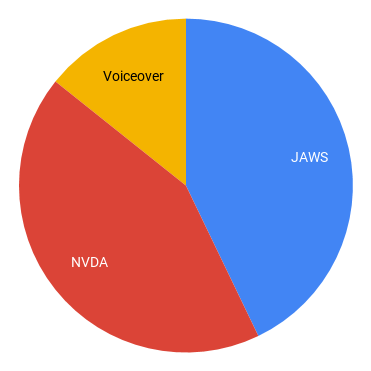
\includegraphics[width=\linewidth]{images/ScreenReader.png}
     \caption{What screen-reader are you using?}
  \end{subfigure}
  \begin{subfigure}[c]{0.3\linewidth}
    \centering
    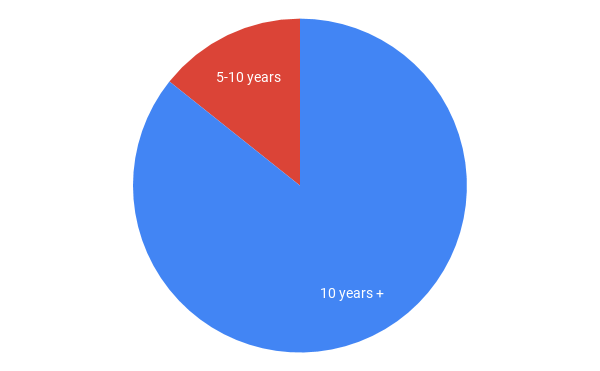
\includegraphics[width=\linewidth]{images/HowLongUsingScreenReader.png}
    \caption{How long have you been using a screen-reader?}
  \end{subfigure}
  \begin{subfigure}[c]{0.3\linewidth}
    \centering
    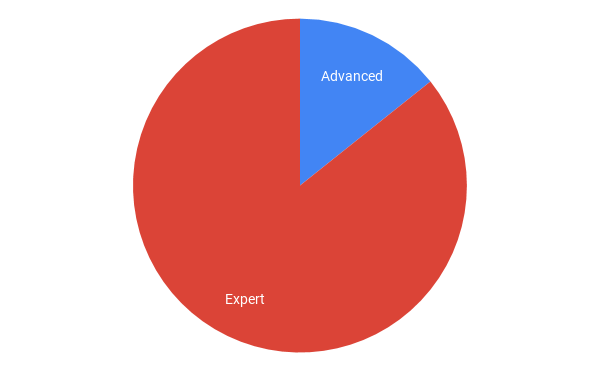
\includegraphics[width=\linewidth]{images/ProficientScreenReader.png}
    \caption{How proficient would you rate yourself using a screen reader?}
  \end{subfigure}
  \caption{Questions about screen-reader usage}
  \label{fig:screenreaderquestions}
\end{figure}

\begin{figure}[H]
  \centering
  \subcaptionbox{Do you find images in web pages accessible?}[.3\linewidth][c]{%
    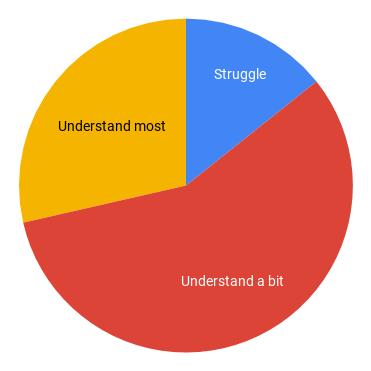
\includegraphics[width=.3\linewidth]{images/ImagesAccessible.png}}\quad
  \subcaptionbox{Do you find tabular data in web pages accessible? }[.3\linewidth][c]{%
    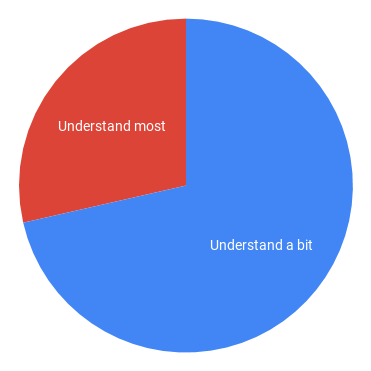
\includegraphics[width=.3\linewidth]{images/TablesAccessible.png}}\quad
  \subcaptionbox{Do you find data visualisations, such as graphs and diagrams, in web pages accessible?}[.3\linewidth][c]{%
    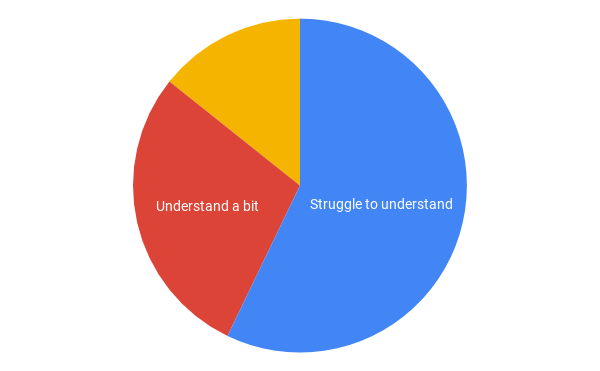
\includegraphics[width=.3\linewidth]{images/DataVizAccessible.png}}\quad
\caption{Questions about visuals and accessibility}
\end{figure}

The post-demo questions had results as follows

\begin{figure}[H]
  \centering
  \subcaptionbox{Did you understand the subject of data that was being presented?}[.3\linewidth][c]{%
    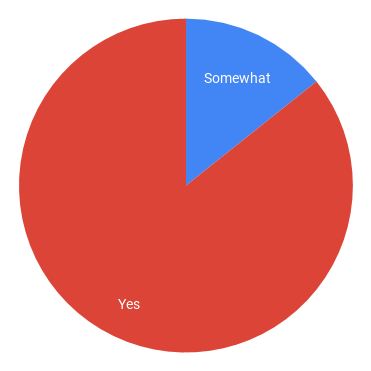
\includegraphics[width=.3\linewidth]{images/UnderstandSubject.png}}\quad
  \subcaptionbox{Did you understand the data that was associated with each data point?}[.3\linewidth][c]{%
    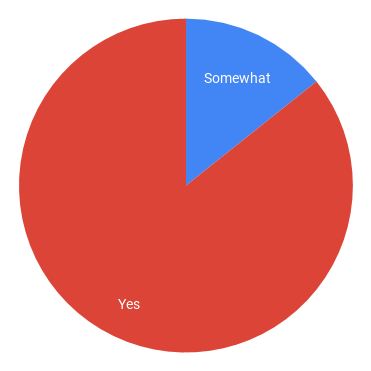
\includegraphics[width=.3\linewidth]{images/UnderstandingDatapoint.png}}\quad
  \subcaptionbox{Was enough information given?}[.3\linewidth][c]{%
    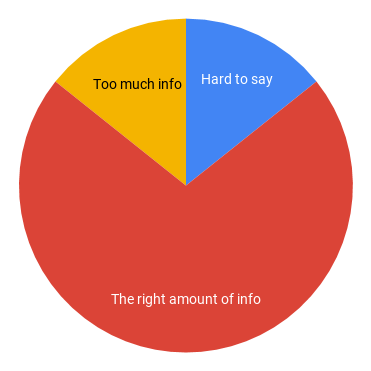
\includegraphics[width=.3\linewidth]{images/InfoGiven.png}}\quad
\caption{Questions about understanding the graphs}
\end{figure}

\begin{figure}[H]
  \centering
  \subcaptionbox{Was it clear how to move between different data points?}[.4\linewidth][c]{%
    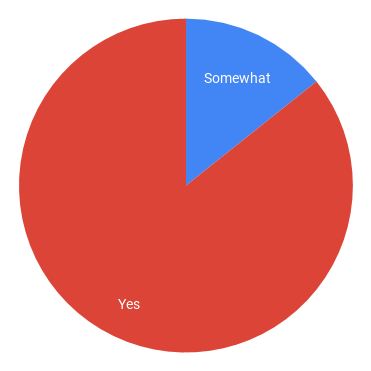
\includegraphics[width=.3\linewidth]{images/NavigatingChart.png}}\quad
  \subcaptionbox{Would you prefer to have different keyboard navigation?}[.4\linewidth][c]{%
    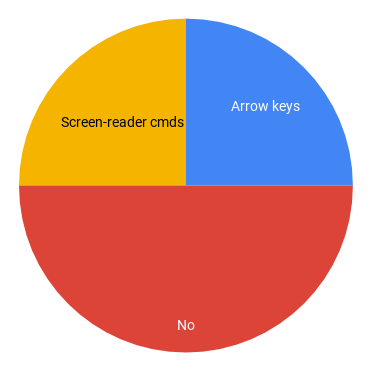
\includegraphics[width=.3\linewidth]{images/ChangeKeys.png}}\quad
\caption{Questions about navigating the graphs}
\end{figure}

Some other qualitative comments from users

\begin{itemize}
    \item It would be useful to have a view where I could use the tab key to browse columns and arrow keys to browse rows
    \item I would have liked to have the graph presented in a way that I could review it in review mode of the screen-reader
    \item I didn't like having \texttt{tabindex} on elements that weren't interactive such as links, buttons, checkboxes
    \item The screen-reader native keys should be used for graph navigation (such as "i" for navigating through \texttt{listitem} elements)
    \item I would have preferred to navigate the graphs using the arrow keys
    \item For the pie chart, it would be useful to have the segment colours included in the information so that I can refer to this when presenting to sighted colleagues
\end{itemize}

\subsection{Analysis}

The background questions gave some simple details on the software the users used -

\begin{itemize}
    \item The most common operating system was \textit{Windows}, and the most common browser was \textit{Chrome}
    \item The \textit{Windows} users were split fairly evenly between those using \textit{Chrome} and \textit{Firefox} - these tend to be the most popular browsers with \textit{Windows} users, so this was to be expected
    \item The users mainly used the screen-readers \textit{JAWS} and \textit{NVDA} - these are the most popular screen-readers on Windows so this was expected
    \item The only user not using \textit{JAWS} or \textit{NVDA} was using \textit{Voiceover} - a popular choice for \textit{MacOS} users due to being native to the operating system
    \item The users were mainly long-term screen-reader users (10+ years), with only one slightly more recent (5-10 years) screen-reader user in the pool
    \item Following on from this, the users mainly rated themselves as "Expert" in their proficiency using a screen-reader to navigate websites
\end{itemize}

The questions asked about whether users currently found different visuals accessible to them - images, tabular data and data visualisation

\begin{itemize}
    \item None of the users said they "Fully Understand" any of these, not even images, implying that there is currently quite a wide disconnect for blind and partially-blind users when it comes to understanding any visuals presented on web pages
    \item A small percentage (29\% for images and tables, 14\% for data visualisations) said that they "Understand Most" for any of these types of visuals
    \item Almost 60\% of users said that they "Struggle to Understand" data visualisations on web pages, so it seems that many developers do not provide adequate descriptions for these, possibly because it can be complex to sum up large amounts of visual data succinctly
\end{itemize}

After the demo, the user was asked some questions about how they found the demo

\begin{itemize}
    \item Most of the users felt that they understood the subject of the graph being presented, and what the value of each individual point was
    \item One user commented that they had some trouble remembering the topic of the graph while browsing, and had to continually return to the title to review this
    \item Most users found that the right amount of information for each data point was presented, with only one user commenting that they found it hard to comment on this without any visual comparison
    \item One user commented that when initially focusing on the graph, a lot of information was read out, but it wasn't too much of a problem for them overall
    \item Most users understood how to navigate through the charts using a keyboard, but some commented that they would have liked their screen-readers browsing methods to be better supported
    \item One user found the user of \texttt{tabindex} on each data point confusing, as they usually associated that with interactive elements on a web page
    \item Most users were fine with using the \texttt{[Tab]} key being used for navigation, but several said that the keyboard arrow keys would also be good navigation options
    \item Some users said that they would have liked some different keyboard navigation systems such as letter keys, especially as many screen-readers have specified shortcuts for navigating through \texttt{listitem} elements such as the \texttt{i} key
\end{itemize}

\subsection{Limitations}

% Didn't test use of colour
% Better study would compare table against graph data

\section{WCAG}

The WCAG guidelines provide a framework for basic evaluation of an accessible page. The following table shows all relevant criteria being fulfilled

\begin{center}
\begin{longtable}{|p{2cm}|p{5cm}|p{2cm}|p{5cm}|}
 \hline
 Num & Name & Done? & Notes \\ [0.5ex]
 \hline \hline
 1.1.1 & Non-text Content & $\text{\rlap{$\checkmark$}}\square$ & All the graphical content has text labels\\
 \hline
 1.2 & Time-based media & $\text{\rlap{$\checkmark$}}\square$ & There is no audio or video content\\
 \hline
 1.3.1 & Info and Relationships & $\text{\rlap{$\checkmark$}}\square$ & Graph data points are made as a \texttt{listitem} to show structure to the user\\
 \hline
 1.3.2 & Meaningful Sequence & $\text{\rlap{$\checkmark$}}\square$ & Data points are in a list in an ordered sequence\\
 \hline
 1.3.3 & Sensory Characteristics & $\text{\rlap{$\checkmark$}}\square$ & Content is suitable for both visual and audio senses\\
 \hline
 1.3.4 & Orientation & $\text{\rlap{$\checkmark$}}\square$ & Not applicable to a smaller image on a web page\\
 \hline
 1.3.5 & Identify Input Purpose & $\text{\rlap{$\checkmark$}}\square$ & There is no user input\\
 \hline
 1.3.6 & Identify Purpose & $\text{\rlap{$\checkmark$}}\square$ & All elements are made with correct HTML tags or assigned ARIA roles\\
 \hline
 1.4.1 & Use of Color & $\text{\rlap{$\checkmark$}}\square$ & All colour used has corresponding text and pattern counterparts\\
 \hline
 1.4.2 & Audio Control & $\text{\rlap{$\checkmark$}}\square$ & There is no audio content\\
 \hline
 1.4.3 & Contrast (Minimum) & $\text{\rlap{$\checkmark$}}\square$ & Descriptive text is high contrast (\textgreater 4.5:1)\\
 \hline
 1.4.4 & Resize Text & $\text{\rlap{$\checkmark$}}\square$ & Text can be resized\\
 \hline
 1.4.5 & Images of Text & $\text{\rlap{$\checkmark$}}\square$ & All text in the graphs is rendered as a \texttt{<text>} tag\\
 \hline
 1.4.6 & Contrast (Enhanced) & $\text{\rlap{$\checkmark$}}\square$ & Descriptive text is high contrast (\textgreater 7:1)\\
 \hline
 1.4.7 & Low or No Background Audio & $\text{\rlap{$\checkmark$}}\square$ & There is no audio content\\
 \hline
 1.4.8 & Visual Presentation & $\text{\rlap{$\checkmark$}}\square$ & There are no blocks of text in the charts\\
 \hline
 1.4.9 & Images of Text & $\text{\rlap{$\checkmark$}}\square$ & All text in the graphs is rendered as a \texttt{<text>} tag\\
 \hline
 1.4.10 & Reflow & $\text{\rlap{$\checkmark$}}\square$ & Text reflows, and the graph may require scrolling but this is allowed due to needing 2-dimensional layout for meaning\\
 \hline
 1.4.11 & Non-text Contrast & $\text{\rlap{$\checkmark$}}\square$ & Adjacent colour blocks have a fairly high contrast (\textgreater 3:1)\\
 \hline
 1.4.12 & Text Spacing & $\text{\rlap{$\checkmark$}}\square$ & Letter spacing is \textgreater 0.12 times the font size, and word spacing is \textgreater 0.16 times the font size\\
 \hline
 1.4.13 & Content on Hover and Focus & $\text{\rlap{$\checkmark$}}\square$ & There is no content triggered by hovering, labels triggered by focus continues to play until the user manually shifts focus\\
 \hline
 2.1.1 & Keyboard & $\text{\rlap{$\checkmark$}}\square$ & All content is operable through a keyboard interface without requiring specific timings\\
 \hline
 2.1.2 & No Keyboard Trap & $\text{\rlap{$\checkmark$}}\square$ & All elements that can receive keyboard focus can have focus moved away using only a keyboard interface\\
 \hline
 2.1.3 & Keyboard (No Exception) & $\text{\rlap{$\checkmark$}}\square$ & All content is operable through a keyboard interface without requiring specific timings\\
 \hline
 2.1.4 & Character Key Shortcuts & $\text{\rlap{$\checkmark$}}\square$ & There are no keyboard shortcuts implemented for letters, punctuations or numbers\\
 \hline
 2.2 & Enough Time & $\text{\rlap{$\checkmark$}}\square$ & There is no content that has a time limit on viewing, contains interruptions, or has timeouts/re-authentication\\
 \hline
 2.3 & Seizures and Physical Reactions & $\text{\rlap{$\checkmark$}}\square$ & There is no animation in the content that could trigger a seizure or physical reaction\\
 \hline
 2.4.1 & Bypass Blocks & $\text{\rlap{$\checkmark$}}\square$ & Each graph has a skip link before presenting any content to the user\\
 \hline
 2.4.2 & Page Titled & $\text{\rlap{$\checkmark$}}\square$ & Applies to the parent web page, not the included divs with graphs\\
 \hline
 2.4.3 & Focus Order & $\text{\rlap{$\checkmark$}}\square$ & Applied to a full page as opposed to single content, but focus order on the graphs is sequential to the elements\\
 \hline
 2.4.4 & Link Purpose (In Context) & $\text{\rlap{$\checkmark$}}\square$ & The only link is the bypass link and this is clearly labelled for all users\\
 \hline
 2.4.5 & Multiple Ways & $\text{\rlap{$\checkmark$}}\square$ & Applies only to locating a web page within a set of web pages\\
 \hline
 2.4.6 & Headings and Labels & $\text{\rlap{$\checkmark$}}\square$ & All headings and labels describe the topic and purpose\\
 \hline
 2.4.7 & Focus Visible & $\text{\rlap{$\checkmark$}}\square$ & The keyboard operable interface has visible indication of where the keyboard focus is\\
 \hline
 2.4.8 & Location & $\text{\rlap{$\checkmark$}}\square$ & User location in a set of webpages only applies to a full web page\\
 \hline
 2.4.9 & Link Purpose (Link Only) & $\text{\rlap{$\checkmark$}}\square$ & All links can have their purpose determined from the link text only\\
 \hline
 2.4.10 & Section Headings & $\text{\rlap{$\checkmark$}}\square$ & The correct HTML sectioning element is used for the graph divs\\
 \hline
 2.5 & Input Modalities & $\text{\rlap{$\checkmark$}}\square$ & There are no user inputs in the charts\\
 \hline
 3.1.1 & Language of Page & $\text{\rlap{$\checkmark$}}\square$ & The default human language of the page will need to be set on the parent page\\
 \hline
 3.1.2 & Language of Parts & $\text{\rlap{$\checkmark$}}\square$ & The human langauge of all the phrases in the content can be programmatically determined\\
 \hline
 3.1.3 & Unusual Words & $\text{\rlap{$\checkmark$}}\square$ & All language is simple English without unusual words\\
 \hline
 3.1.4 & Abbreviation & $\text{\rlap{$\checkmark$}}\square$ & There are no abbreviations included\\
 \hline
 3.1.5 & Reading Level & $\text{\rlap{$\checkmark$}}\square$ & All language is simple English with a reading level lower than secondary education\\
 \hline
 3.1.6 & Pronunciation & $\text{\rlap{$\checkmark$}}\square$ & There are no words included without context that would need help being pronounced\\
 \hline
 3.2.1 & On Focus & $\text{\rlap{$\checkmark$}}\square$ & When a user interface component receives focus it does not initiate a change of context\\
 \hline
 3.2.2 & On Input & $\text{\rlap{$\checkmark$}}\square$ & There is no user input that would cause a change of context\\
 \hline
 3.2.3 & Consistent Navigation & $\text{\rlap{$\checkmark$}}\square$ & Navigation mechanisms being repeated applies between different web pages in a set of web pages\\
 \hline
 3.2.4 & Consistent Identification & $\text{\rlap{$\checkmark$}}\square$ & All graph components on a page can be identified consistently\\
 \hline
 3.2.5 & Change on Request & $\text{\rlap{$\checkmark$}}\square$ & There are no changes in context initiated without user request\\
 \hline
 3.3 & Input Assistance & $\text{\rlap{$\checkmark$}}\square$ & There is no user input that would require helping the user to avoid and correct mistakes\\
 \hline
 4.1.1 & Parsing & $\text{\rlap{$\checkmark$}}\square$ & All HTML elements have start and end tags, unique IDs, no duplicated attributes and are nested correctly\\
 \hline
 4.1.2 & Name, Role, Value & $\text{\rlap{$\checkmark$}}\square$ & All user interface components have roles set either using correct HTML tags or assigning ARIA roles\\
 \hline
 4.1.3 & Status Messages & $\text{\rlap{$\checkmark$}}\square$ & There are no status attributes on any of the chart elements\\
 \hline
\end{longtable}
\end{center}

\section{Open-Source Contributions}

In the process formulating syntax for my solution, I did a lot of reading around the HTML specification \cite{htmlspec} in order to understand the HTML Accessibility API Mappings. One of the key sources of documentation for web development is the MDN Web Docs \cite{mdndocs}, which provide comprehensive web standards and other information for web developers.

While reading through specifications and the MDN web docs, it became clear that there were undocumented syntactical features in the \texttt{Document} interface, and so I made some open-source contributions to the documentation there.

% LATER - more detail on contributions

\chapter{Conclusion and Future Work}

Overall the solution produced did fairly well in user testing, with most users giving positive feedback around understanding the data presented and being able to navigate through the graph.

However, it was clear from user comments that there is a wide variety of ways that users want data presented to them, and any single solution will not be accessible to everyone. To produce a solution that is truly accessible to the majority of people, there will need to be multiple data ordering and navigational methods available to the user within one chart. To have a solution that works consistently among major browsers and operating systems will also require a lot of careful use of syntax, and this may not be very easily possible until future years when HTML, ARIA and SVG specifications work uniformly across different software.

As with any user-facing work, a lot of user-testing is required to develop a solution that works well with a variety of people. The testing for this project only covered blind and partially-blind users, whereas future testing should also cover colour-blind users and those with motor and cognitive disabilities.

I hope to have the opportunity to develop the library further, there are several key areas that could be developed

\begin{itemize}
    \item Expanding to more graph types - most graphing libraries allow several dozen types of common graphs to be produced
    \item Allowing customisable navigation
        \begin{itemize}
            \item Several users in the study voiced that they would like different key combinations to be used
            \item Having arrow keys used may be more intuitive for users, but will require some more complex technical work, as there is very little consistency between different browsers in defining arrow key interactions on web pages
            \item It may be useful for developers to be able to define navigational keys themselves, especially if they would like consistency between the graphs and other parts of the parent page
            \item Developers may wish to have the option to pick between several specified navigation options, such as "tab key", "arrow keys", "letter keys" or turn off keyboard navigation altogether
            \item Several users mentioned that their screen-readers have native keys for navigating through lists, so it will be a good idea to also integrate this into the solution
        \end{itemize}
    \item Customising colours
        \begin{itemize}
            \item Being able to choose the colours on the graphs will make it easier to make graphs that are in line with other presented visuals, or with brand guidelines
            \item However due to the WCAG restrictions on colour contrast, it may be the case that developers have to pick from specific colour palettes
        \end{itemize}
\end{itemize}

The solution I presented relies on navigating through the entire graph to understand each data point. This would work for smaller datasets, but users with cognitive disabilities may struggle to remember the graph topic as they navigate through multiple data points, and someone wanting to find a specific value may have to read through several unwanted values to get there.

Visuals such as graphs are mainly presented as such because they give the viewer the ability to quickly see trends and relations, and find relevant information easily, e.g. a line graph can be a good way of illustrating that there is a strong upward trend over time, or that a value has been steady over a period of time.

Another way of thinking about making graphical data accessible is to allow users to query certain aspects of the graph, such as having an interface that allows questions like "what was the trend between years 2000 and 2010", so this may be a possible way to create accessible data visualisations.

% LATER - rewrite?
% - Goals I had for the project, and did I fulfill them (aim for 3/4 goals?)

\chapter{Glossary}

% LATER - review glossary words

When talking about web accessibility, it is useful to highlight some key terms

\BlankLine
%
\glsaddall
\printglossary[nonumberlist]

\printbibliography

% \chapter{Appendix}

% LATER - move WCAG table here?
% LATER - raw user survey results?
% LATER - change both headings that are WCAG to differing ones? i.e. "implementing WCAG" and "WCAG compliance"

\end{document}

%-----------------------------------------------------------------------
% Plan
%-----------------------------------------------------------------------

% WAI-ARIA compliant
% Screen-reader
% Insight on stats?
% Able to tab through (each bar/bubble?)
% Different patterns for colour-blind users
% Stick to few types - bars, pie, line, stacked bars?
% For line talk about trends, for bar/pie talk about most "X is most, do you want to hear more?"
% - Things like speed compared to other libraries such as d3
